%%%%%%%%%%%%%%%%%%%%%%%%%%%%%%%%%%%%%%%%%%%%%%%%%%%%%%%%%%%%%
% Example of an article for the RBCA Journal                %
%                                                           %
% Please note that whilst this template provides a          %
% preview of the typeset manuscript for submission, it      %
% will not necessarily be the final publication layout.     %
%                                                           %
% a4paper: UK paper size toggle                             %
% alpha-refs: author-year citation and bibliography toggle  %
% RBCA_v2.0: RBCA latex class
%%%%%%%%%%%%%%%%%%%%%%%%%%%%%%%%%%%%%%%%%%%%%%%%%%%%%%%%%%%%%

\documentclass[alpha-refs,brazilian]{RBCA_v2.0}

%%% Place your packages here
\usepackage{subfig}                                         %Biblioteca para Múltiplas Figuras
%\usepackage{censor}                                        %Biblioteca para Avaliação Cega
%\usepackage[tablename=Quadro]{caption}                     %Biblioteca para renomear Quadros


%%% Paper title
\title{Avaliação e Remodelagem de um Jogo Sério para Prevenção do Abuso Sexual Infantil}
\titleother{Evaluation and Redesign of a Serious Game to Child Sexual Abuse Prevention}

%%% The orcid number of authors (\orcid) is optional.       %Agora é obrigatório
\author[1]{Alexandre Mendonça Fava \orcid{0000-0001-5605-2326}}
\author[1]{Carla Diacui Medeiros Berkenbrock \orcid{0000-0001-9854-4046}}
\author[1]{Adilson Vahldick \orcid{0000-0002-0442-3735}}

\affil[1]{Universidade do Estado de Santa Catarina - UDESC}

%%% Author e-mails
\authnote{\authfn{1}alexandre.fava@hotmail.com; carla.berkenbrock@udesc.br; adilson.vahldick@udesc.br}

%%% "Short" author for running page header - until 3 authors
%\runningauthor{First, Second \& Third}

%%% "Short" author for running page header - more than 3 authors
\runningauthor{Fava, Berkenbrock \& Vahldick}    

%%% Paper category:
%%% English  : Original paper,  Experience Report     or Tutorial
%%% Português: Artigo original, Relato de experiência ou Tutorial
\papercat{Artigo original}

%%% Editor should only set information about the issue journal and the paper
\jvolume{13}                                                % volume number
\jissue{1}                                                  % issue number
\jyear{2021}                                                % edition year
\jmonth{April}                                              % edition month

\setcounter{page}{1}                                        % number of the first page of the paper
\firstpage{1}
\jid{9999}                                                  % paper ID 

\jrec{yyyy-mm-dd}                                           % date of article submission
\jrev{yyyy-mm-dd}                                           % date of final paper revision
\jacc{yyyy-mm-dd}                                           % date of paper accepted

\begin{document}
\begin{frontmatter}
	
\maketitle
\thispagestyle{empty}


%The Abstract (200 words maximum) should be structured to include the following details: \textbf{Background}, the context, and purpose of the study; \textbf{Results}, the main findings; \textbf{Conclusions}, summary, and potential implications. Please minimize the use of abbreviations and do not cite references in the abstract.
\begin{Abstract}                                            % abstract in english
    In 2018, the National Ombudsman's Office for Human Rights received over than 17 thousand sexual assault reports on Disque 100 hotline targeting victims of up to 18 years of age. As result, some game-based strategies were been developed to fight against child sexual abuse. One collaborative game comes up with a strategy for prevention of the sexual assault crimes. The game was evaluated by the present research in order to verify its quality, in both the educational and ergonomic sense. A preliminary analysis of the game pointed out contradictions against the games and experts recommendations. Therefore, a deeper evaluation of the game was carried out and modifications were proposed to treat such issues, leading to the redesign of the game according to the available literature. In the end, both versions were compared using the MEEGA evaluation methodology. The evaluation process executed concluded a better motivation and user experience for the new version of the game. As a result, this research brings a potentially promising game for the prevention of child sexual violence.
\end{Abstract}

%Keyword1; keyword 2; keyword 3 (Three to five keywords representing the main content of the article, in alphabetic order)
\begin{keywords}
    Evaluation; Serious Games; Prevention; Child Sexual Abuse
\end{keywords}

%O Resumo (com até 200 palavras) deverá ser estruturado para abordar os seguintes detalhes: \textbf{Background}, o contexto e propósito do estudo; \textbf{Resultados}, os principais encontrados; \textbf{Conclusões}, um breve resumo do trabaho e as implicações em potencial. Por favor, evite, na medida do possível, o uso de abreviaturas e não cite referências no resumo.
\begin{resumo}
    Para o ano de 2018, o Disque 100, canal de denúncia oficial do Ministério da Mulher, da Família e dos Direitos Humanos, totalizou 17.093 denúncias de violência sexual contra crianças e adolescentes. Em resposta a violência infantil, surgiram algumas estratégias baseadas em jogos para a prevenção do abuso sexual contra os menores. Entre os jogos, destaca-se um jogo pela sua abordagem colaborativa no combate à violência sexual infantil no Brasil. O jogo foi avaliado pela presente pesquisa com o intuito de assegurar sua qualidade, tanto em níveis educacionais, quanto em níveis ergonômicos. A análise revelou divergências entre o jogo e recomendações presentes na literatura acerca da criação e modelagem de jogos. Tais divergências serviram como base para a criação de uma nova versão do jogo. Ao final, ambas as versões foram comparadas por meio da metodologia avaliativa MEEGA. O processo avaliativo realizado constatou uma melhor motivação e experiência dos usuários para nova versão do jogo. Como resultado, essa pesquisa traz um jogo potencialmente promissor para a prevenção da violência sexual infantil. 
\end{resumo}

%Palavra-chave 1; palavra-chave 2; palavra-chave 3 (De três a cinco palavras-chave que representem os principais tópicos do artigo, em ordem alfabética)
\begin{palavras_chave}
	Avaliação; Jogos Sérios; Prevenção; Violência Sexual Infantil
\end{palavras_chave}

\end{frontmatter}
\clearpage


\section{Introdução}
O Brasil possui a terceira maior população carcerária do mundo, apenas atrás dos Estados Unidos da América e da China \citep{mabud2019evaluating}. Em 2018 o Departamento Penitenciário Nacional contabilizou uma população de 725.332 presos, com 44\% (327.535) dos presos encarcerados em decorrência de crimes contra o patrimônio, 28\% (210.409) por crimes relacionados às drogas, 12\% (91.865) por crimes contra a pessoa e 4\% (32.509) por crimes de cunho sexual, estando os demais presos enquadrados em outras categorias \citep{departamento2018levantamento}.

Os crimes de cunho sexual são definidos pelo Código Penal brasileiro como `crimes contra a dignidade sexual'. Dentre eles, é possível citar: assédio, rufianismo, tráfico de pessoas e estupro \citep{codigo2018crimes}. Quando praticados, tais atos são capazes de sequelar suas vítimas tanto fisicamente, quanto psicologicamente. Das sequelas psicológicas destaca-se: transtorno mental, transtorno de comportamento, estresse pós-traumático, tendência suicida e depressão \citep{cerqueira2014estupro}. Fisicamente, entre as sequelas estão: dificuldades para caminhar, edemas, baixo controle dos esfíncteres, contusões e fraturas \citep{bocardi2003gravidez, florentino2015possiveis}.

Os crimes de violência sexual demonstram preocupação não apenas por causa das suas sequelas, mas também, pelo fato de mais da metade de suas vítimas serem menores de idade. Somente no ano de 2018, o Disque 100\footnote{O Disque 100 funciona diariamente, 24 horas por dia, incluindo sábados, domingos e feriados. Existem três opções para registrar sua denúncia: Disque 100, aplicativo Proteja Brasil e Ouvidoria Online (Disponível em: \underline{\url{https://www.humanizaredes.gov.br/ouvidoria-online/}})} registrou um total de 17.093 denúncias de violência sexual contra crianças e adolescentes, sendo 78,5\% das denúncias relacionadas especificamente ao abuso sexual infantil \citep{ouvidoria2019balanco}. Além disso, já é de notório conhecimento de estudiosos na área que todos os dados sobre a violência sexual estão subnotificados, o que implica que a quantidade de criminosos denunciados é inferior à quantidade real de criminosos existentes \citep{world2016world}.

Diante do problema e das consequências da violência sexual, inúmeras medidas surgiram focadas principalmente no encarceramento de criminosos, como a operação \textit{Darknet} da Polícia Federal \citep{policia2017operacao}. Todavia, esse tipo de estratégia demonstra-se ineficaz em resolver o problema da violência sexual infantil pelo simples fato de ser uma medida de correção e não de prevenção. A dificuldade infantil em manifestar a violência sofrida acaba prejudicando as medidas tomadas pelas organizações policiais \citep{brito2015estupro}. Políticas de prevenção demonstram-se mais efetivas, como o Programa Educacional de Resistência às Drogas e à Violência (PROERD) que capacita alunos de todo o Brasil contra o uso de drogas \citep{vasconcelos2018eficacia}.

\pagebreak

Visando o combate contra a violência sexual infantil, \cite{diocesano2018jogo} apresentam uma proposta preventiva de jogo educacional para instruir e capacitar as crianças no assunto, ajudando-as a compreender melhor o tema e ensinando-as a realizar denúncias. O jogo em questão intitula-se \textbf{Infância Segura}. Esse jogo foi analisado pela presente pesquisa para assegurar que os conteúdos ministrados estariam devidamente adequados para seu público alvo (crianças entre 5 e 6 anos de idade). Como resultado, a revisão bibliográfica revelou divergências entre o jogo educacional desenvolvido e recomendações para criação e modelagem de jogos presentes na literatura, o que por sua vez culminou no desenvolvimento de uma segunda versão do jogo \textbf{Infância Segura}, supostamente mais adequada ao público infantil em relação a proposta original do jogo. 

Tanto o jogo original \citep{diocesano2018jogo}, quanto a nova versão desenvolvida pela presente pesquisa foram submetidas a testes de usuários. Os testes foram realizados por intermédio da metodologia de análise de jogos intitulada \textit{Model for the Evaluation of Educational Games} (MEEGA) \citep{savi2011model}, com a finalidade de mensurar a experiência dos usuários em relação a ambos os jogos. Dito isso, informa-se que o presente artigo encontra-se estruturado da seguinte maneira: a \cref{secao:TrabalhosRelacionados} apresenta os trabalhos relacionados com esta pesquisa no que diz respeito a avaliação de jogos sérios; a \cref{secao:InfanciaSeguraOriginal} descreve o jogo desenvolvido por  \cite{diocesano2018jogo}; a \cref{secao:EstudoArte} relata a análise pedagógica e técnica realizada sobre o jogo; a \cref{secao:InfanciaSegura2.0} apresenta o novo jogo proposto por esta pesquisa; a \cref{secao:Experimentos} relata os experimentos realizados com ambos os jogos; a \cref{secao:Resultados} apresenta os resultados alcançados; e a
\cref{secao:ConsideracoesFinais} traz as considerações finais do artigo.


\section{Trabalhos Relacionados}\label{secao:TrabalhosRelacionados}

Jogos são utilizados como instrumento recreativo ou como instrumento educacional há anos \citep{clark1970serious}. Em virtude disso, surgiram inúmeros modelos e manuais para a avaliação de jogos. A avaliação de jogos é uma atividade essencial no \textit{design} instrucional, pois permite avaliar a eficácia pedagógica do jogo, constatando se  cada lição do jogo consegue cumprir com aquilo que foi planejado para ele \citep{montilva2002method, padron2007towards}. Dito isso, a presente seção apresenta alguns jogos avaliados. 

Os jogos sérios \textbf{Conquistando com o Resto} e \textbf{Desafios com Palitos} são jogos acadêmicos desenvolvidos na Universidade de Pernambuco (UPE), sendo eles a virtualização de jogos já utilizados de forma positiva no ensino da Matemática. Utilizando três diferentes abordagens para a avaliação de jogos, \cite{oliveira2015avaliaccao} constataram dificuldades por parte dos jogadores em compreender o objetivo do jogo \textbf{Conquistando com o Resto}. Todavia, o jogo \textbf{Desafios com Palitos} não apresentou problemas, se destacando inclusive de forma positiva no ensino de algarismos romanos, conversão de valores e raciocínio lógico.

\newpage
\newcommand\x{3.1 cm}
\newcommand\xx{3.2 cm}
\newcommand\y{4.2 cm}
\newcommand\yy{3 cm}
\newcommand\z{1.9 cm}
\newcommand\zz{6 cm}

\begin{table*}[bh]
\renewcommand\arraystretch{2.4}
\renewcommand{\tablename}{Quadro}
\caption{Trabalhos Relacionados} 
\label{quadro:TrabalhosRelacionados}
\centering
\scalebox{0.75}{
\begin{tabular}{    
    |>{\centering\arraybackslash}m{\x}
    |>{\centering\arraybackslash}m{\xx}
    |>{\centering\arraybackslash}m{\y}
    |>{\centering\arraybackslash}m{\yy}
    |>{\centering\arraybackslash}m{\z}
    |>{\arraybackslash}m{\zz}|
    }
\cline{1-1}\cline{2-2}\cline{3-3}\cline{4-4}\cline{5-5}\cline{6-6}
    \multicolumn{1}{|p{\x}|}{\cellcolor{blue!25}\centering \textbf{Jogo}} &
    \multicolumn{1}{p{\xx}|}{\cellcolor{blue!25}\centering \textbf{Objetivo}} &
    \multicolumn{1}{p{\y}|}{\cellcolor{blue!25}\centering \textbf{Metodologia(s) Adotada(s)}} &
    \multicolumn{1}{p{\yy}|}{\cellcolor{blue!25}\centering \textbf{Modelo de Avaliação}} &
    \multicolumn{1}{p{\z}|}{\cellcolor{blue!25}\centering \textbf{Grupo (Perfil)}} &
    \multicolumn{1}{p{\zz}|}{\cellcolor{blue!25}\centering \textbf{Resultados}}
    \\
\cline{1-1}\cline{2-2}\cline{3-3}\cline{4-4}\cline{5-5}\cline{6-6}
    \textbf{Desafios com Palitos} &
    Ensinar matemática &
    Learning Object Review Instrument (LORI); GameFlow; Níveis de avaliação de Kirkpatrick &
    Escala de Likert &
    10 pessoas \hspace{1 mm} (10 a 12 anos) &
    Sem problemas constatados
    \\
\cline{1-1}\cline{2-2}\cline{3-3}\cline{4-4}\cline{5-5}\cline{6-6}
    \textbf{Conquistando com o Resto} &
    Ensinar matemática &
    \textit{Learning Object Review Instrument} (LORI); GameFlow; Níveis de avaliação de Kirkpatrick &
    Escala de Likert &
    10 pessoas \hspace{1 mm} (10 a 12 anos) &
    Objetivo pouco intuitivo
    \\
\cline{1-1}\cline{2-2}\cline{3-3}\cline{4-4}\cline{5-5}\cline{6-6}
    \textbf{Esquadrão 192} &
    Ensinar sobre o AVC (Acidente Vascular Cerebral) &
    Testes de Retenção &
    Entrevista; Escala visual de humor Pick-A-Mood (PAM); Grupo Focal &
    43 pessoas \hspace{1 mm} (8 a 12 anos) &
    A música agitada não agradou os participantes, os quais tiveram dificuldades com o \textit{mouse} e dificuldades em alternar entre os periféricos: \textit{mouse} e teclado
    \\
\cline{1-1}\cline{2-2}\cline{3-3}\cline{4-4}\cline{5-5}\cline{6-6}
    \textbf{EducaCorpoHumano3D} &
    Ensinar sobre o corpo humano &
    \textit{Digital Game-Based Learning} (DBGL) &
    Fun Toolkit (Smileyometer, Again Again Table) &
    36 pessoas \hspace{1 mm} (9 a 13 anos) &
    Observou-se desinteresse por grande parte do grupo em dedicar tempo para a leitura das instruções do jogo
    \\
\cline{1-1}\cline{2-2}\cline{3-3}\cline{4-4}\cline{5-5}\cline{6-6}
    \textbf{InspSoft} &
    Apoiar o ensino de inspeção de \textit{software} &
    \textit{Model for the Evaluation of Educational Games} (MEEGA) &
    Escala de Likert &
    16 pessoas \hspace{1 mm} (idade não encontrada) &
    O jogo não progride em um ritmo adequado
    \\
\cline{1-1}\cline{2-2}\cline{3-3}\cline{4-4}\cline{5-5}\cline{6-6}
    \textbf{Jogo Original} &
    Ensinar sobre a prevenção da violência sexual infantil &
    \textit{Model for the Evaluation of Educational Games} (MEEGA) &
    Escala de Likert &
    2 pessoas \hspace{1 mm} (6 e 12 anos) &
    Notou-se dificuldade na compreensão das regras de algumas fases, assim como dificuldade na execução das fases. Além disso, constatou-se rejeição ao visual do jogo
    \\
\cline{1-1}\cline{2-2}\cline{3-3}\cline{4-4}\cline{5-5}\cline{6-6}
    \textbf{Novo Jogo} &
    Ensinar sobre a prevenção da violência sexual infantil &
    \textit{Model for the Evaluation of Educational Games} (MEEGA) &
    Escala de Likert &
    2 pessoas \hspace{1 mm} (6 e 12 anos) &
    Foi observado a necessidade de um botão para a releitura dos áudios
    \\
\hline
\end{tabular}}
\end{table*}

O jogo digital nomeado de \textbf{Esquadrão 192} foi desenvolvido pelo Laboratório de Ergodesign de Interfaces, Experiência do Usuário e Usabilidade (LEXUS/UFRN) para ajudar crianças a diagnosticarem os sintomas do Acidente Vascular Cerebral (AVC). Usando testes de humor, testes de retenção e entrevistas grupais, \cite{limeira2015avaliaccao} mostraram que o jogo possibilita maior fixação do conteúdo aprendido, do que a apresentação em forma de desenho animado. %Também foi constatado que o fator desafiador em algumas partes do jogo, demonstrou-se como uma boa ferramenta de engajamento, tornando a ferramenta mais imersiva. 
Como recomendações de melhoria \cite{limeira2015avaliaccao} sugerem a necessidade da dublagem associada ao texto escrito por causa das dificuldades de leitura e interpretação pelas crianças.

O jogo sério intitulado \textbf{EducaCorpoHumano3D}, desenvolvido no Laboratório de Mídia e Conhecimento da Universidade Federal de Santa Catarina (UFSC), tem como principal foco o ensino da anatomia humana para turmas do ensino fundamental. Embasados em técnicas de usabilidade e Digital Game-Based Learning (DBGL) \cite{rombaldi2016educacorpohumano3d} perceberam que o ambiente 3D (três dimensões) do jogo é melhor recebido pelos alunos do que as imagens estáticas 2D (duas dimensões) de livros didáticos.

O jogo \textbf{InspSoft} é um jogo sério que visa apoiar o ensino de inspeção de \textit{softwares}. \cite{lopes2012avaliaccao} não encontraram grandes problemas através da metodologia de \cite{savi2011model}, concluindo que o jogo contribuiu positivamente para que os jogadores desenvolvessem seus conceitos no processo de aprendizagem da inspeção de \textit{software}, apontando como óbice, a progressão inadequada do jogo.

%A revisão bibliográfica realizada a nível nacional não revelou pesquisas relacionadas a avaliação de jogos voltados no combate a violência sexual infantil. Nesse sentido. a revisão bibliográfica acabou por revelar somente o jogo \textbf{CriançaProtegida} \citep{carrara2018criancca}, o qual foca-se no combate a violência sexual infantil, assim como o jogo \textbf{Infância Segura}. Todavia, nenhum dos jogos aparentam já terem sido avaliados por outros estudos até o presente momento.

Um compilado dos artigos relacionados se faz presente no Quadro \ref{quadro:TrabalhosRelacionados}. Na primeira coluna intitulada de \textbf{Jogo} é apresentado o nome do jogo, seguido pelo seu \textbf{Objetivo}, segunda coluna. \textbf{Metodologia(s) Adotada(s)} remete as diferentes estratégias usadas para a avaliação dos jogos; já o \textbf{Modelo de Avaliação}, corresponde à forma como o grupo base teve sua experiência avaliada. Subsequentemente, a coluna \textbf{Grupo (Perfil)} quantifica as dimensões do grupo avaliado definindo em parênteses a faixa etária. Por fim, a coluna \textbf{Resultados} traz observações acerca da análise do jogo em questão.

Todos os artigos apresentados \citep{oliveira2015avaliaccao, limeira2015avaliaccao, rombaldi2016educacorpohumano3d, lopes2012avaliaccao} seguiram uma determinada metodologia para avaliação do jogo. Nesse sentido, salienta-se que o presente artigo não elenca jogos relacionados com a violência sexual infantil, justamente pelo fato das pesquisas na área, envolvendo tais jogos, serem conduzidas por metologias avaliativas voltados ao ensino e aprendizado e não ao jogo em si. Por tal razão, tais pesquisas não foram contempladas no presente estudo bibliográfico: \citep{jones2010being, AnnaErgebnisse2012, jones2020serious}. Entretanto, observou-se que o modelo \textit{Model for the Evaluation of Educational Games} (MEEGA) agrega teorias da área de \textit{design} instrucional e educação \citep{savi2011model}. Devido a essa condição e a possibilidade de personalização do modelo ao contexto do jogo, optou-se por este modelo para avaliação do jogo Infância Segura 1.0 \citep{diocesano2018jogo}. Salienta-se que a avaliação ocorreu apenas após uma análise preliminar do jogo, resultando assim no desenvolvimento do novo Infância Segura 2.0 pela presente pesquisa, o qual passou pelo mesmo processo avaliativo. 

%Não existem jogos, em caráter nacional nessa temática (a presente seção buscou trazer jogos nacionais) e os jogos existentes no exterior conduziram suas metologias avaliativas direcionado ao ensino e não a outros critérios de usabilidade e agradabilidade, por tal razão, não foram contempladas no presente estudo bibliográfico


\section{Jogo Original}\label{secao:InfanciaSeguraOriginal}

O jogo sério \textbf{Infância Segura} visa prevenir o abuso sexual infantil por meio da conscientização e educação de crianças na temática em questão. O jogo foi desenvolvido no campus de Joinville na Universidade do Estado de Santa Catarina (UDESC), com colaboração do Conselho Tutelar de Joinville e do Laboratório Educação e Sexualidade (LabEduSex) do Centro de Educação a Distância (Cead).

O jogo se baseia no Modelo 3C de colaboração, possibilitando assim a comunicação, cooperação e a coordenação do professor \citep{pimentel2006modelo}. Salienta-se então que o jogo em questão é destinado tanto para os alunos quanto para os professores, conforme pode ser observado na \cref{fig:JogoOriginal}.

\begin{figure}[h]
  \centering
  \frame{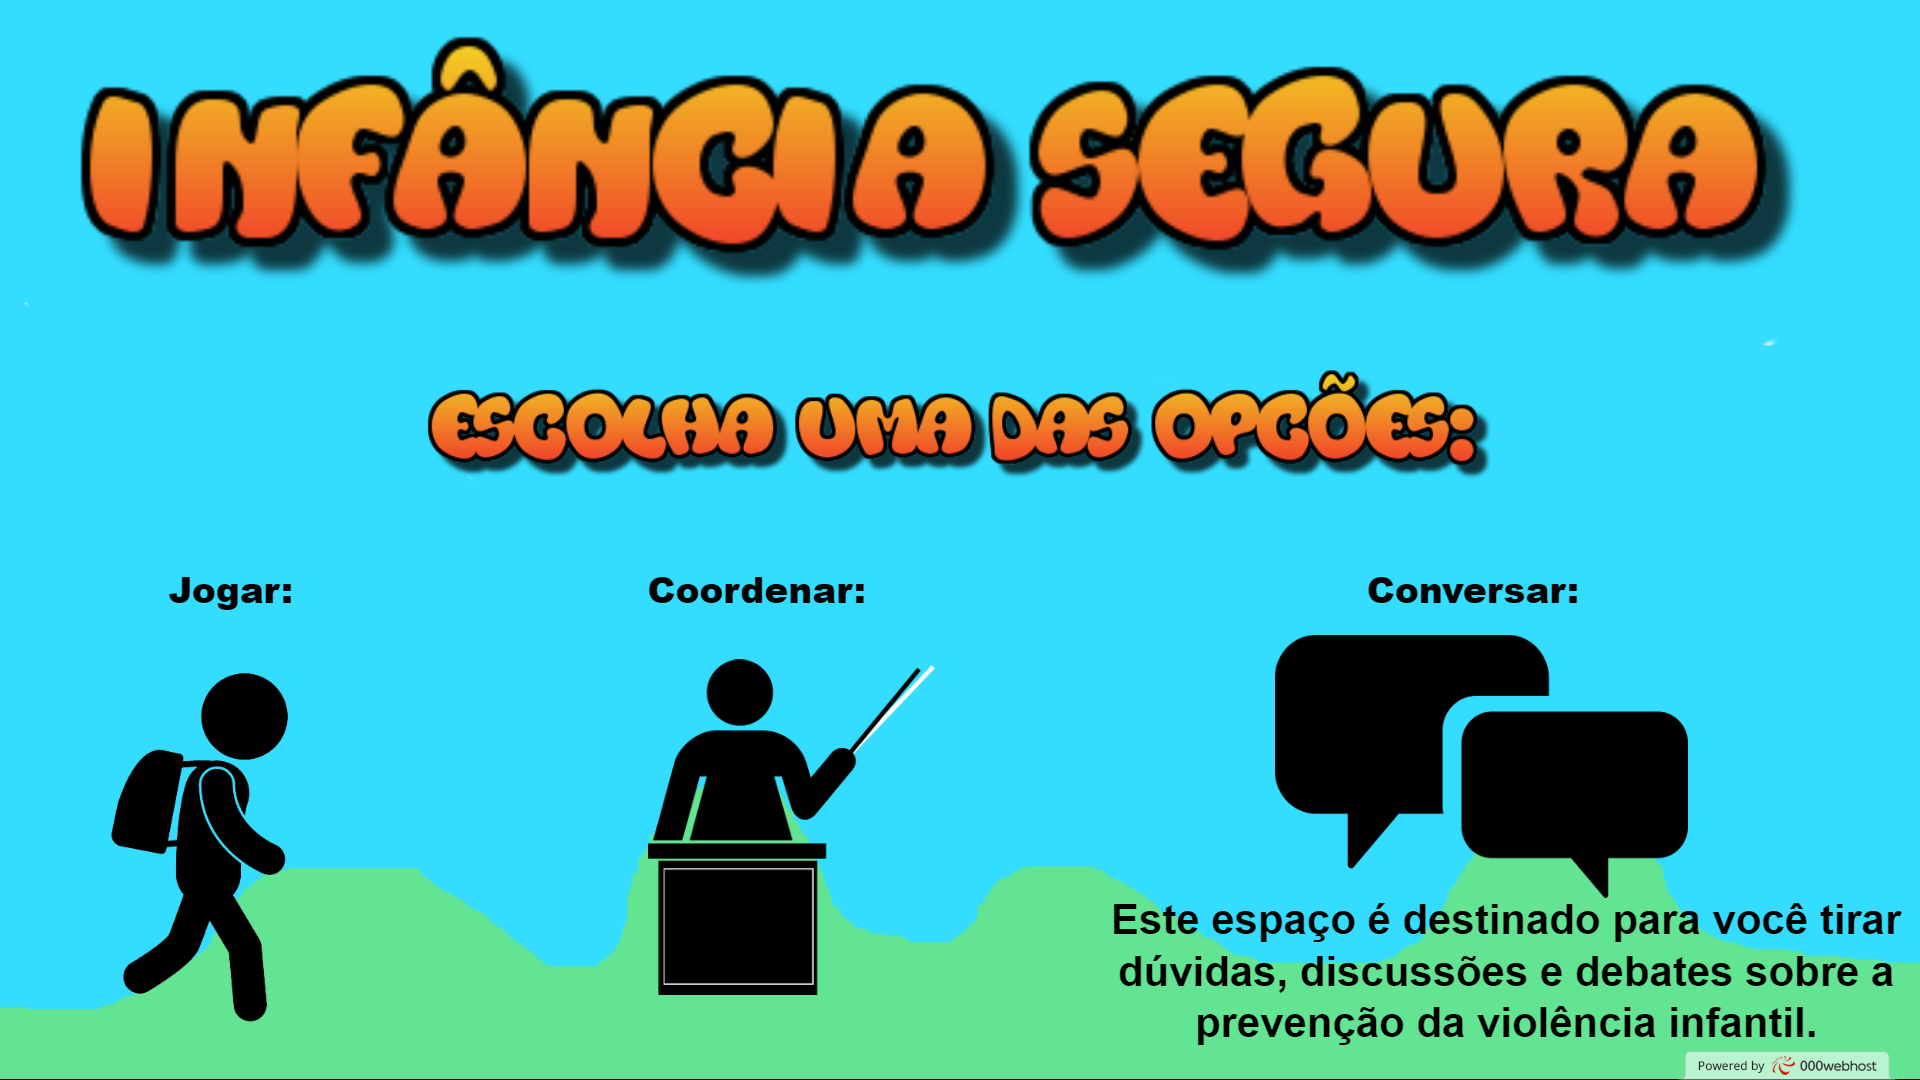
\includegraphics[width=\linewidth]{JogoOriginal/MenuJogo.png}}
  \caption{Tela Principal do \textbf{Infância Segura 1.0}}
  \label{fig:JogoOriginal}
\end{figure}

A \cref{fig:JogoOriginal} mostra a tela principal do jogo, local onde o usuário pode escolher entre três ações: \textbf{Jogar}, \textbf{Coordenar} e \textbf{Conversar}. Cada ação é responsável por uma parte substancial da aplicação, com cada escolha levando o usuário a um ecrã distinto.

A \cref{subsecao:Jogar} trata sobre os aspectos do jogo voltados exclusivamente para o público infantil (opção \textbf{Jogar}), enquanto a \cref{subsecao:Coordenar} aborda os aspectos do jogo relacionados aos educadores (opção \textbf{Coordenar}). A opção \textbf{Conversar} é um espaço compartilhado para os jogadores tirarem dúvidas e promoverem debates sobre os conteúdos ministrados e aprendidos no jogo, similar a uma sala de bate-papo.

\subsection{Jogar}\label{subsecao:Jogar}

A atual seção destaca os principais pontos do jogo, relativos ao jogador. Após selecionar a opção \textbf{Jogar}, a aplicação carrega uma tela de requisição nominal. A criança tem acesso as fases do jogo apenas após sua identificação. Cabe mencionar que as fases do jogo são ministradas de maneira linear não permitindo o jogador alternar entre as fases. A linearidade do jogo é mostrada em maiores detalhes no diagrama de atividade do jogador apresentado na \cref{fig:DiagramaJogar}.

\begin{figure}[h]
  \centering
  \frame{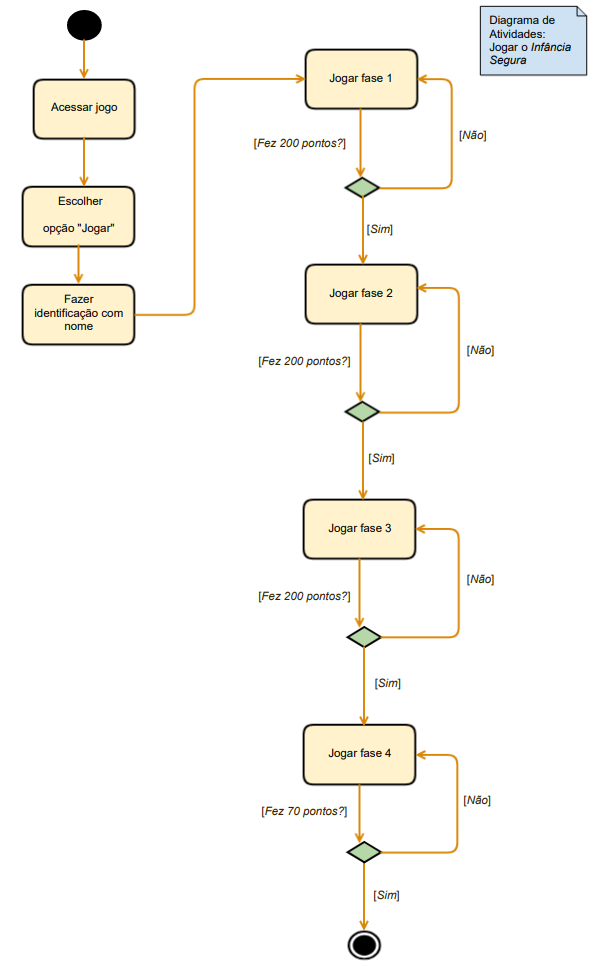
\includegraphics[width=\linewidth]{JogoOriginal/AtividadesJogador.png}}
  \caption{Diagrama de Atividades do Jogador \citep{diocesano2018jogo}} 
  \label{fig:DiagramaJogar}
\end{figure}

\pagebreak

O diagrama de atividade do jogador apresentado na \cref{fig:DiagramaJogar}, demonstra a relação entre as atividades cabíveis ao jogador, onde a transição entre as atividades é resultado direto das ações da criança. Cada fase do jogo visa ministrar um conteúdo específico, relacionado de alguma forma com a prevenção da violência sexual. Todas as quatro fases do jogo são apresentadas na \cref{fig:FasesJogo}, estando todas as fases dubladas.

A \textbf{fase 1} trata das partes íntimas e não íntimas do corpo da criança. Nessa etapa um avatar virtual introduz para o jogador quais são as partes íntimas e não íntimas. Ao final, são apresentadas as regras de um eventual jogo de caixas, sendo uma caixa para as partes íntimas e outra caixa para as partes não íntimas. Quando o jogo se inicia de fato (\cref{fig:FasesJogo1}), partes do corpo começam a cair no cenário, neste momento o jogador deve usar sua destreza e atenção para colocar as partes do corpo nas caixas certas.

\newpage

A \textbf{fase 2} aborda sobre toques bons e ruins. Nessa etapa o mesmo avatar virtual se apresenta, porém agora ensinando sobre as formas corretas e incorretas de toque. Depois da introdução, são apresentadas as regras de um outro jogo, com um menino andando por um cenário. Durante o jogo (\cref{fig:FasesJogo2}), várias imagens aparecem assincronamente, as imagens de toques bons devem atingir um personagem de boné vermelho. Quando aparecem imagens de `toques ruins' o jogador deve clicar no personagem para que seja emitida uma magia para eliminar a imagem de `toque ruim'.

A \textbf{fase 3} leciona sobre a interação com pessoas. Nessa etapa o avatar virtual se apresenta explicando sobre a interação com desconhecidos. Em seguida (\cref{fig:FasesJogo3}), o jogador deve pilotar uma aeronave, seguindo a mesma estrutura de regras da fase anterior, entretanto com movimentação bidimensional, com as imagens `boas' (toques bons) tendo que encostar a nave e as imagens `ruins' (toques ruins) tendo que ser eliminadas por ela.

A \textbf{fase 4} apresenta o tópico \textit{Internet}. Nessa fase o avatar virtual ensina sobre os termos de uso de algumas redes sociais, interação com estranhos e medidas de segurança. Ao final o jogador é colocado em frente a um \textit{Quiz} (\cref{fig:FasesJogo4}) tendo que responder `Sim' ou `Não', para determinadas situações que ocorrem na internet.

 \begin{figure}[h]
  \centering
  \subfloat[Fase 1: partes íntimas e não íntimas]{\frame{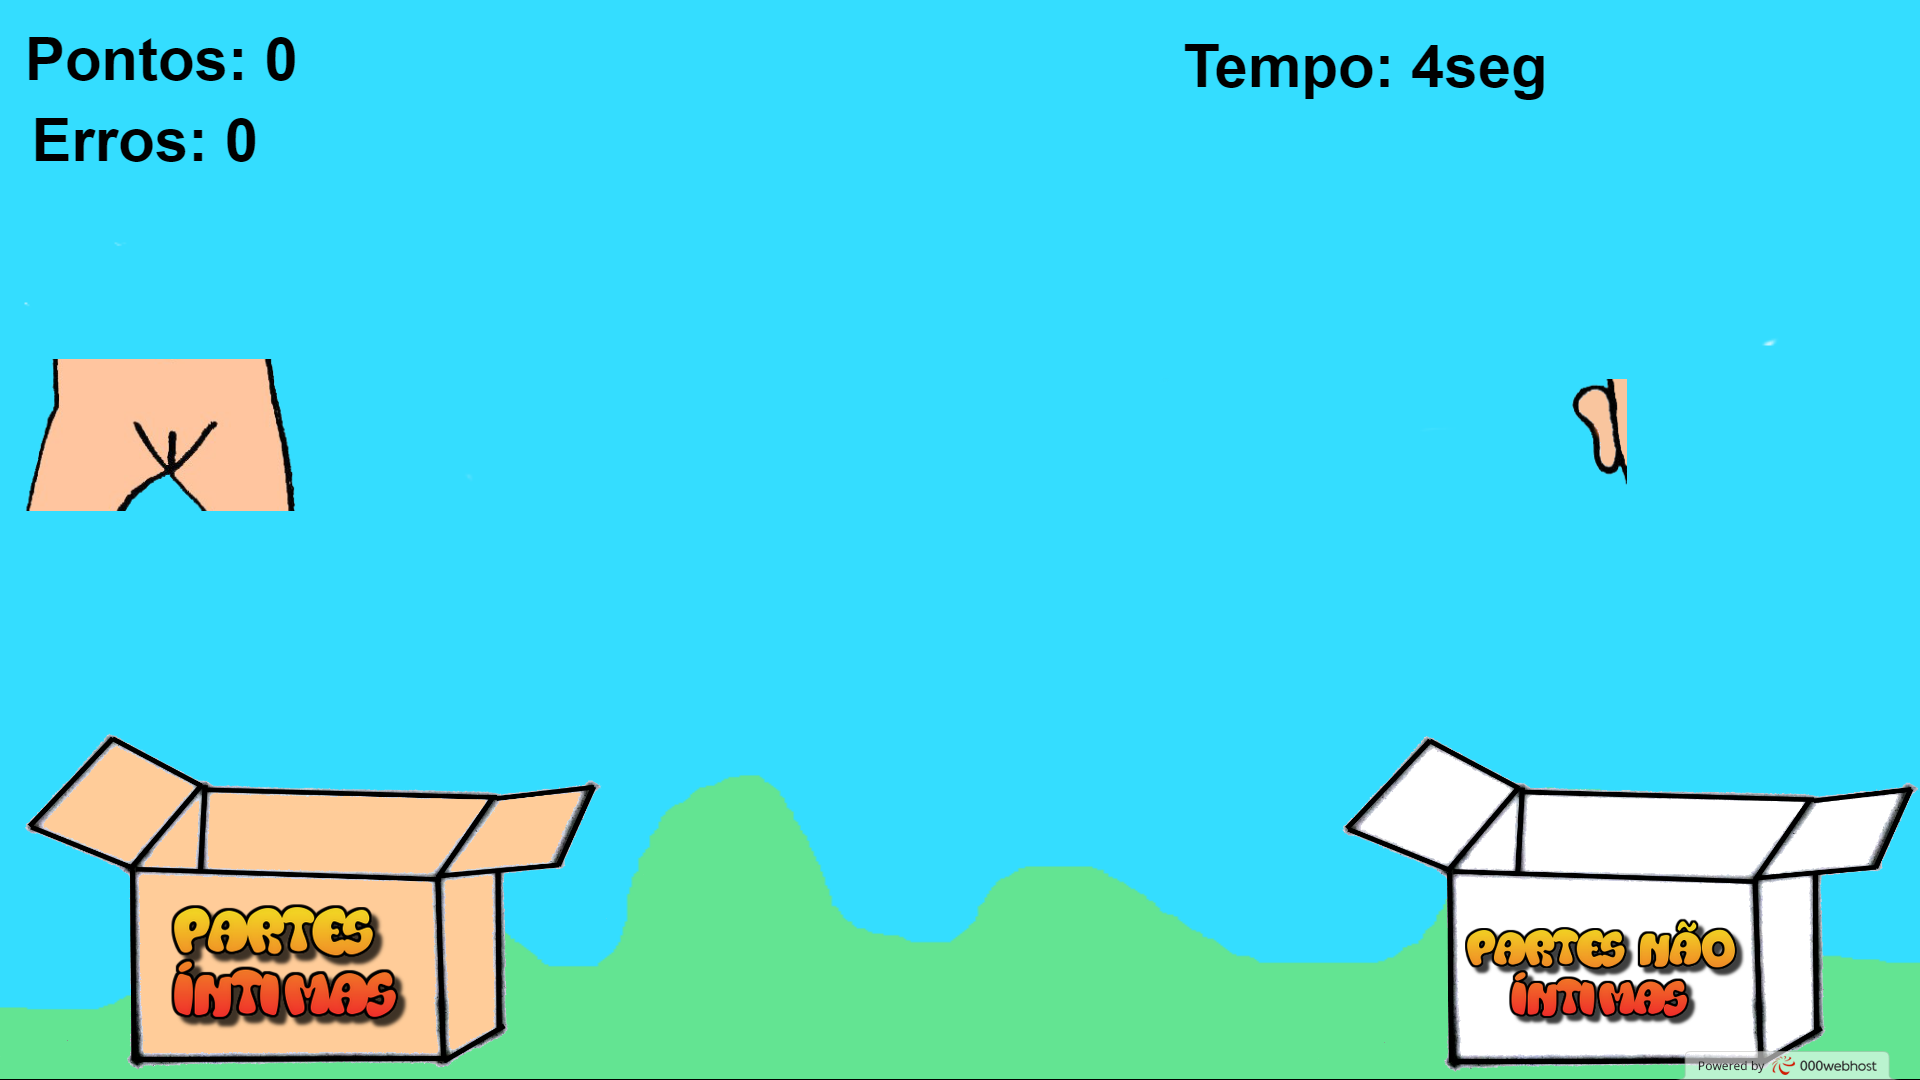
\includegraphics[width=0.49\linewidth]{JogoOriginal/Fase1.png}}\label{fig:FasesJogo1}}\hspace{0.1mm}
  \subfloat[Fase 2: toques bons e ruins]{\frame{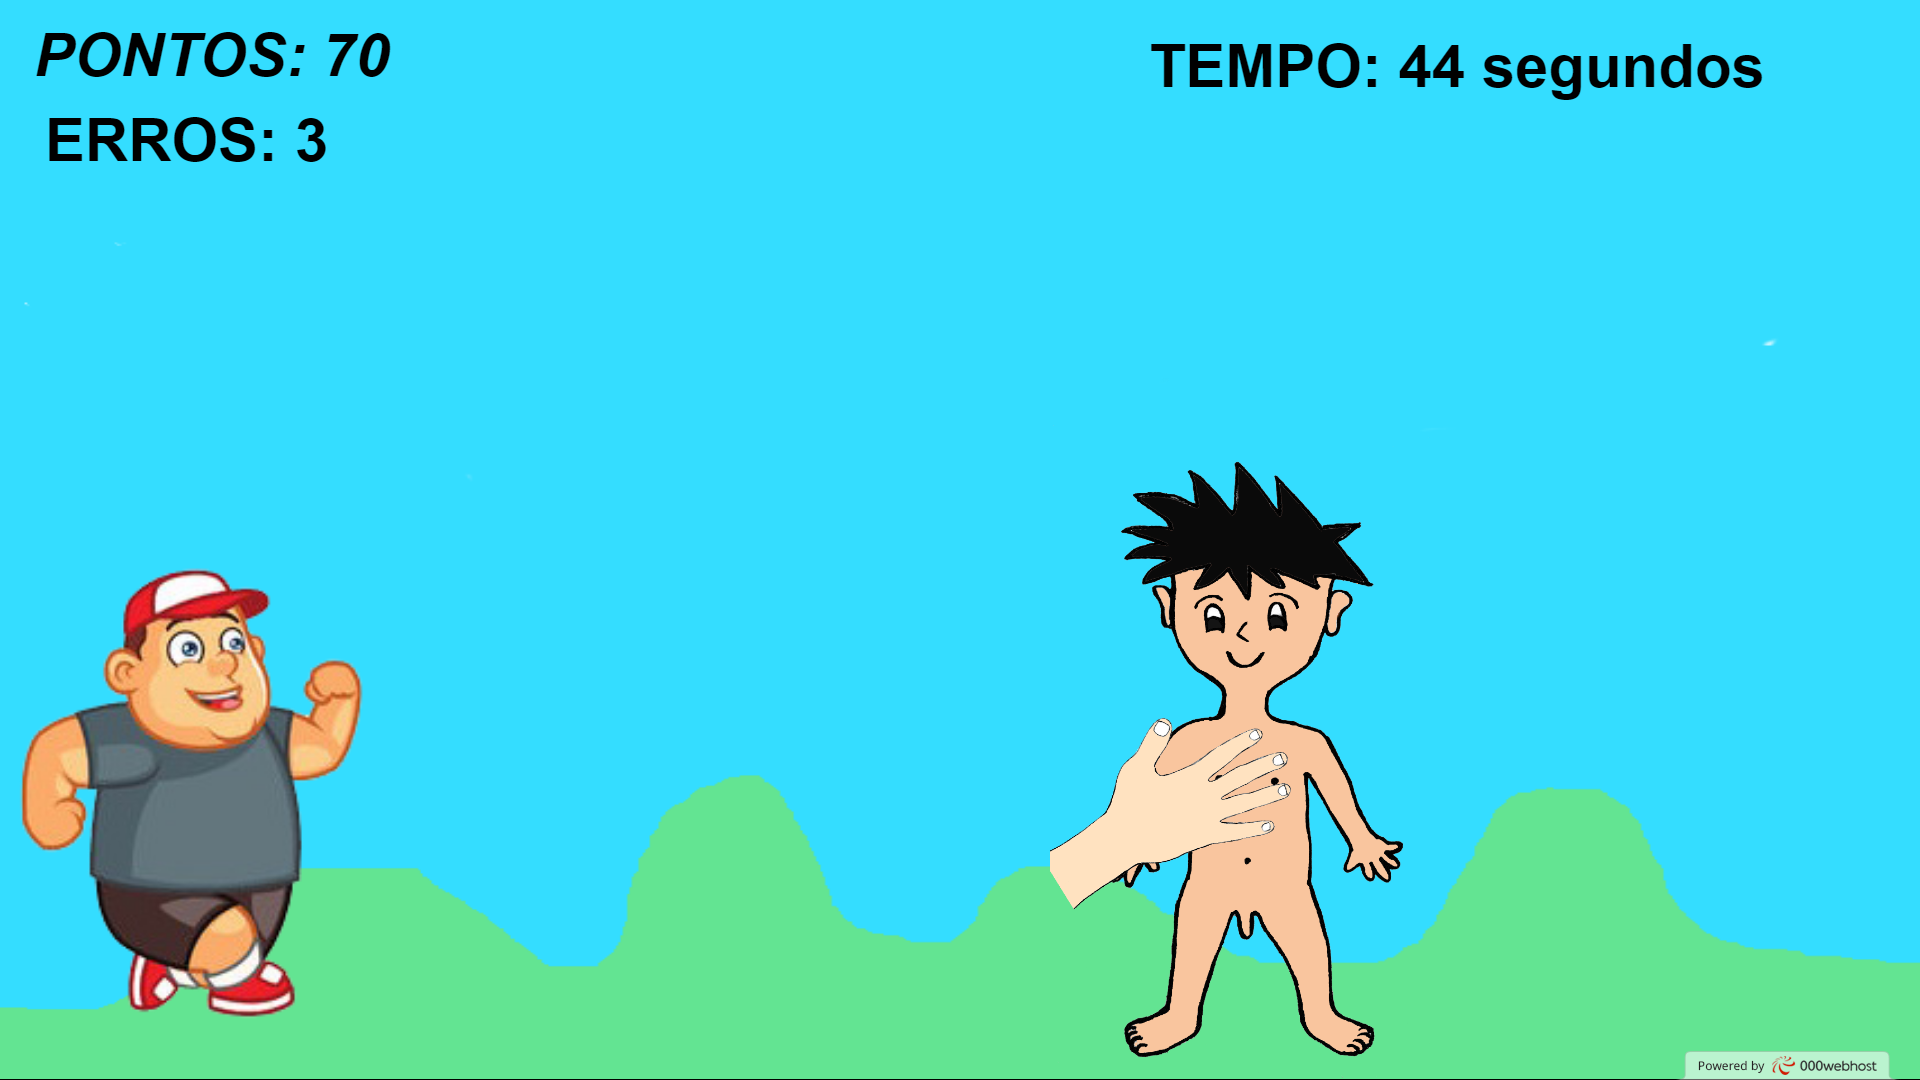
\includegraphics[width=0.49\linewidth]{JogoOriginal/Fase2.png}}\label{fig:FasesJogo2}}
  \hfill
  \subfloat[Fase 3: interação com pessoas]{\frame{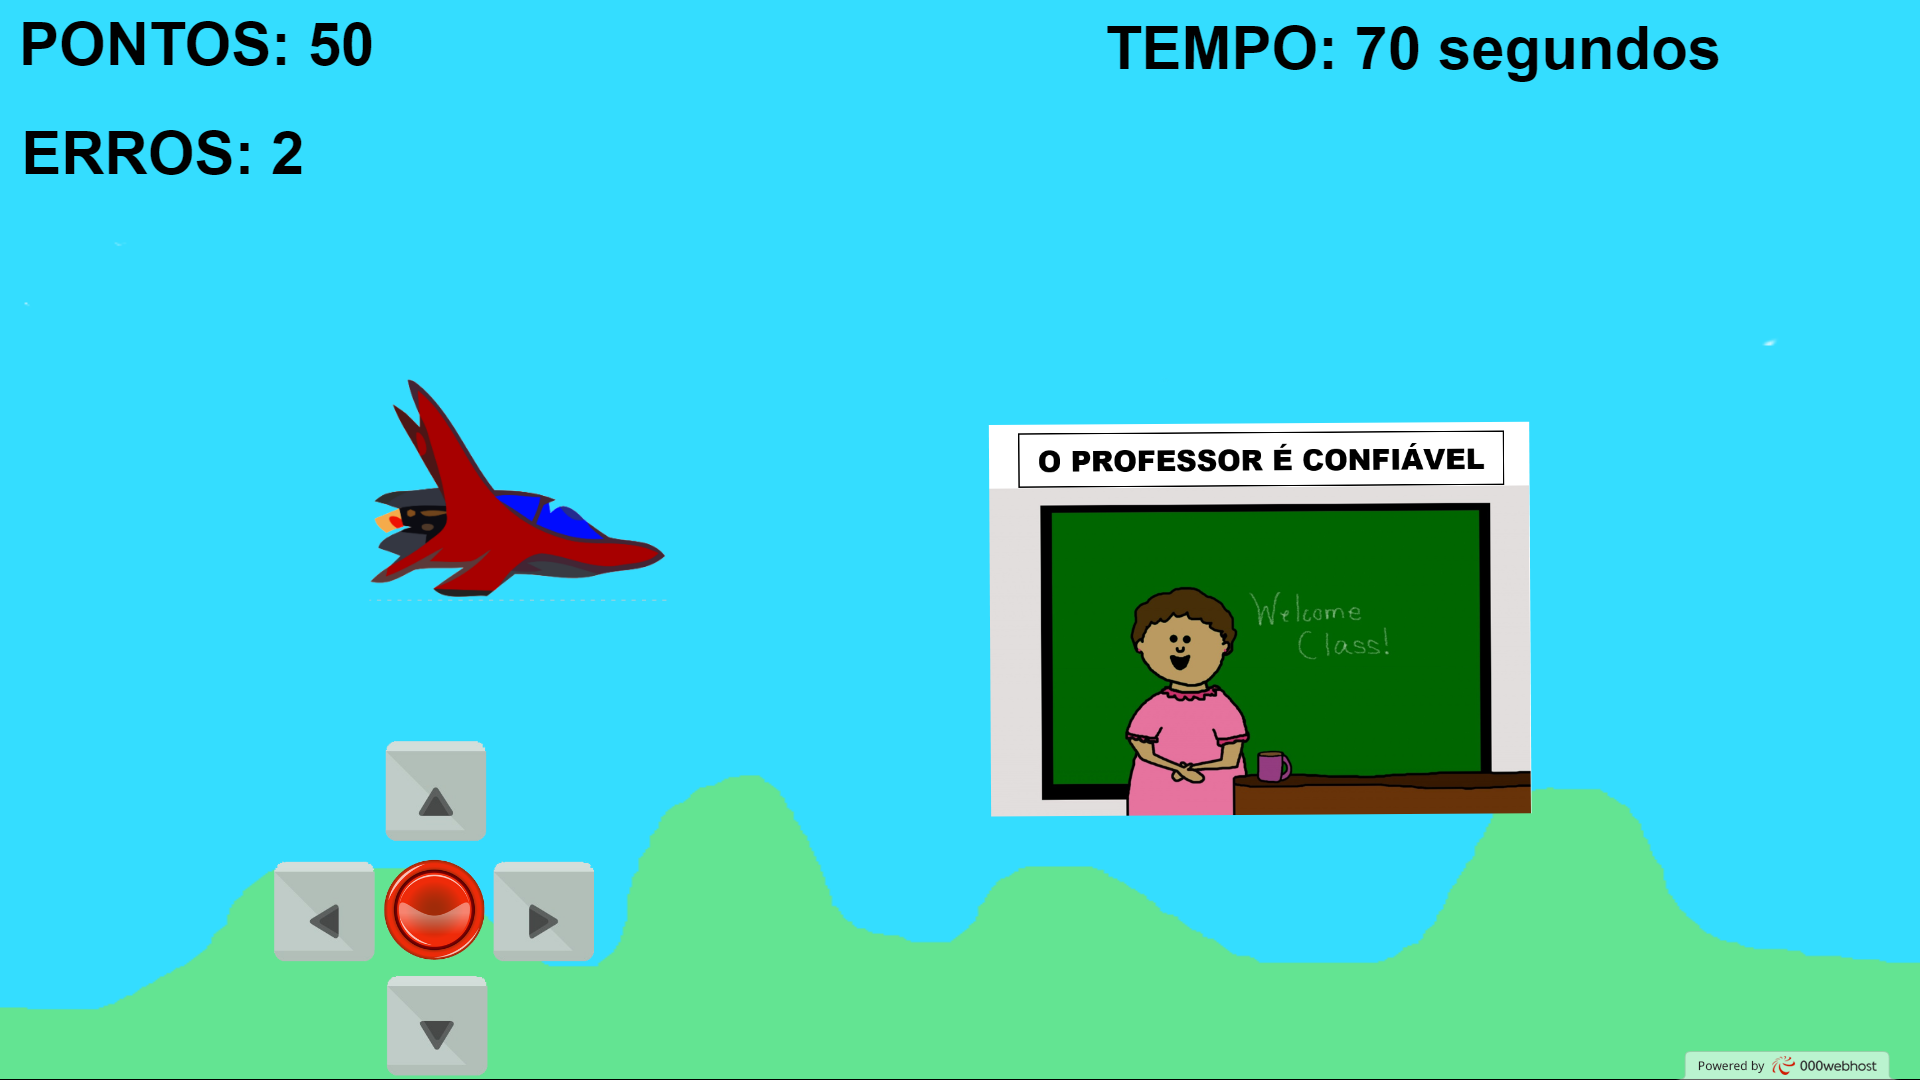
\includegraphics[width=0.49\linewidth]{JogoOriginal/Fase3.png}}\label{fig:FasesJogo3}}\hspace{0.1mm}
  \subfloat[Fase 4: interação na \textit{Internet}]{\frame{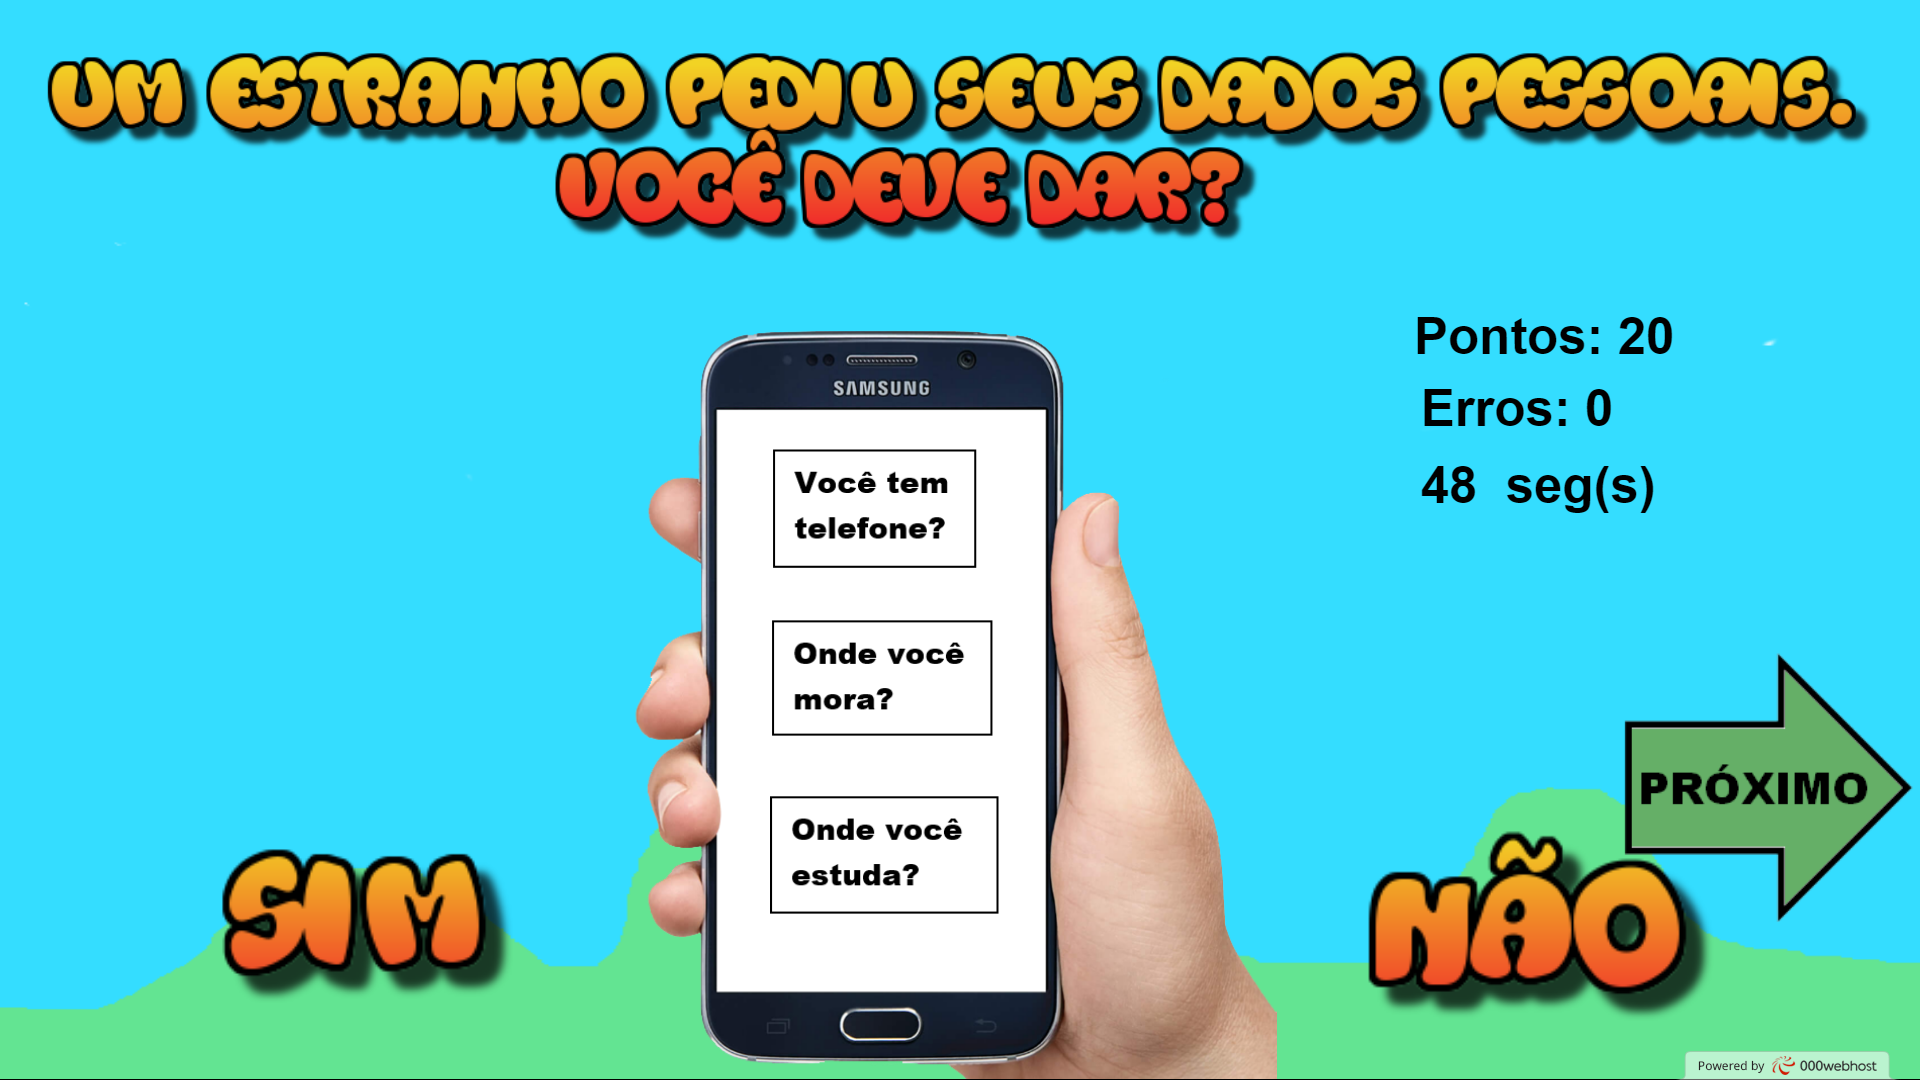
\includegraphics[width=0.49\linewidth]{JogoOriginal/Fase4.png}}\label{fig:FasesJogo4}}
  \caption{Telas das fases do Jogo}
  \label{fig:FasesJogo}
\end{figure}

Após a \textbf{fase 4}, uma tela final é carregada ao jogador, permitindo-o recomeçar ou sair da aplicação. Destaca-se nesse sentido, que nenhuma informação registrada durante o uso do jogo (\textit{Local Store}) prevalece após o jogo ser fechado. Em outras palavras, a criança precisará passar pelas etapas de autenticação manualmente sempre que iniciar o jogo. Além disso, uma vez que os conteúdos tenham sido ministrados, a criança não possui a liberdade de intercambiar entre as fases do jogo, ou seja, no cenário onde a criança deseja jogar o \textit{Quiz} do jogo (\textbf{fase 4}), ela obrigatoriamente, precisa passar por todas as fases anteriores.


\subsection{Coordenar}\label{subsecao:Coordenar}

A atual seção destaca os principais pontos do jogo voltados para o educador. Após selecionar a opção \textbf{Coordenar}, a aplicação carrega uma outra tela de opções, transcrita na \cref{fig:PrincipalCoordenar}. Salienta-se que não existe nenhuma barreira que impeça o acesso de uma criança ou outrem na presente área.

\begin{figure}[h]
  \centering
  \frame{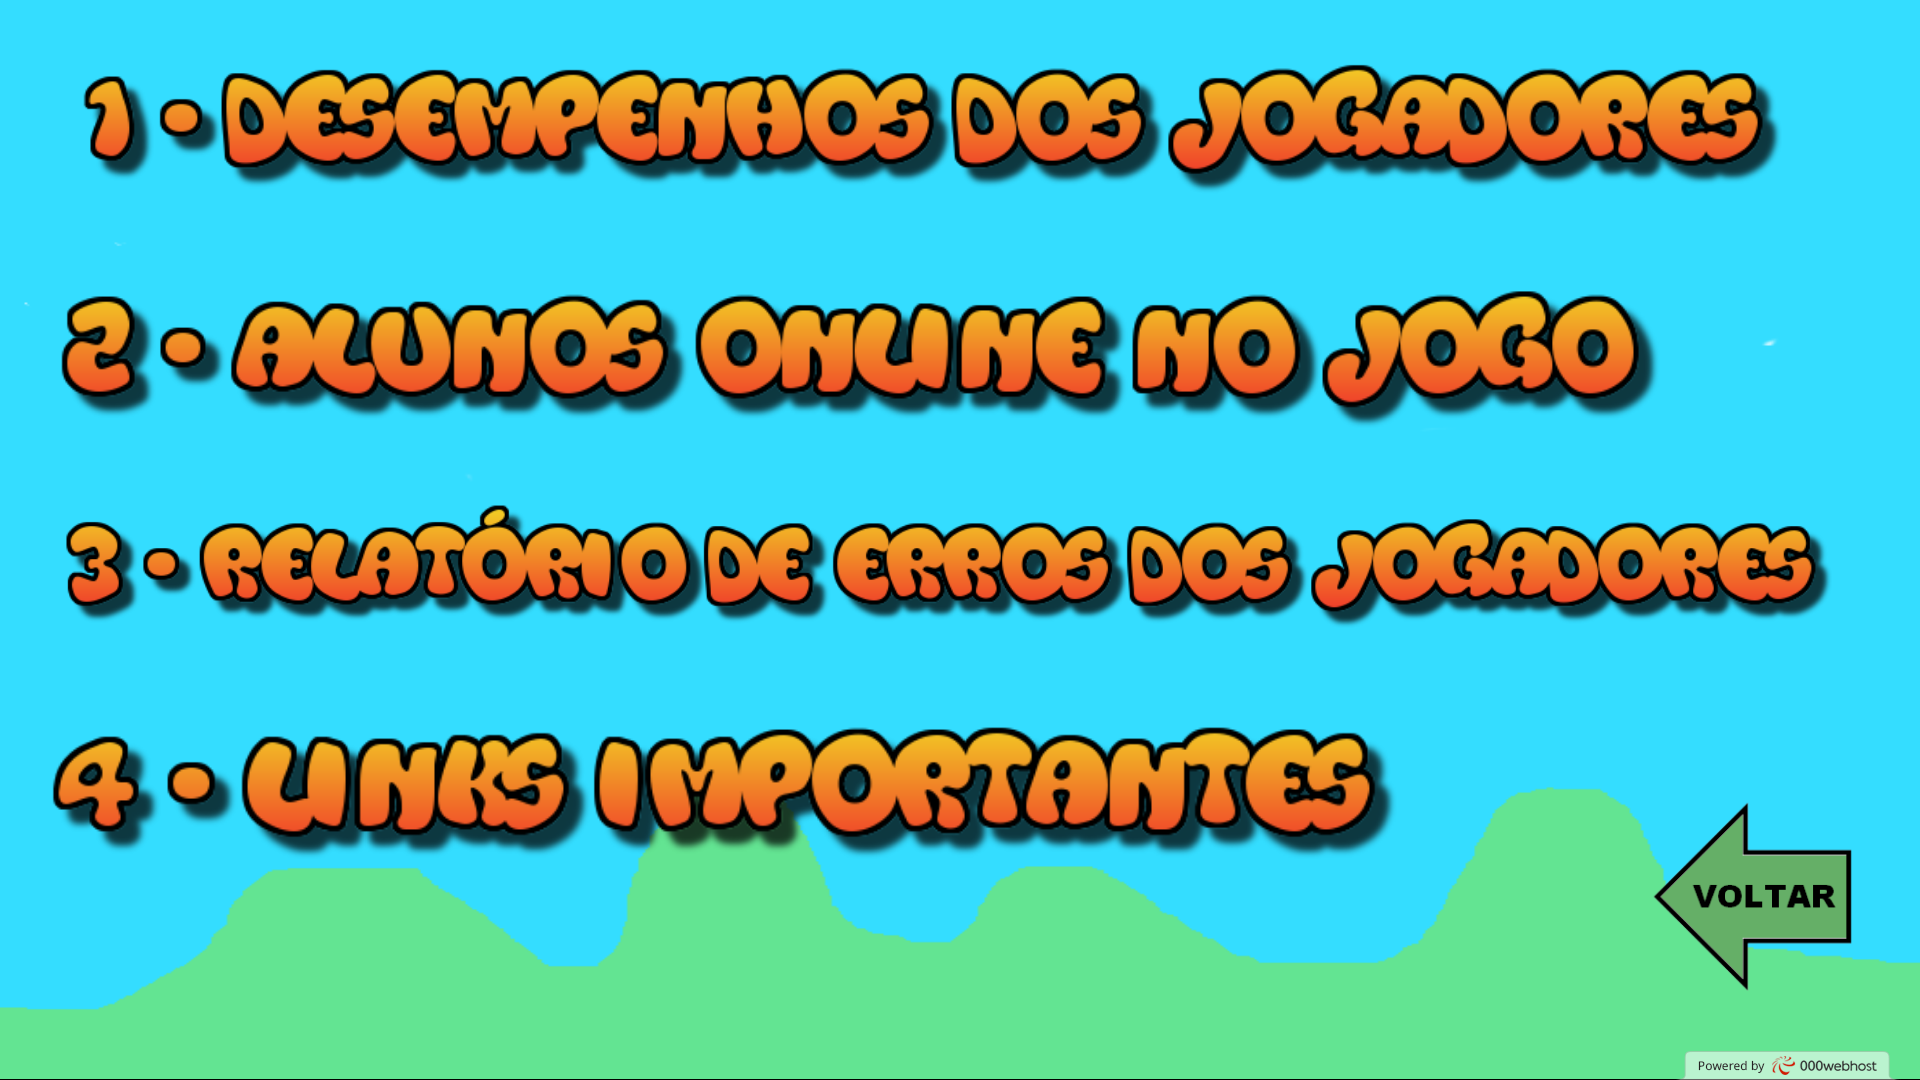
\includegraphics[width=\linewidth]{JogoOriginal/MenuCoordenador.png}}
  \caption{Tela Principal do Educador}
  \label{fig:PrincipalCoordenar}
\end{figure} 

Na zona de opções da \cref{fig:PrincipalCoordenar} o professor pode escolher entre: Desempenho dos jogadores; Alunos \textit{online} no jogo; Relatório de erros dos jogadores; \textit{Links} importantes; e Voltar. Após selecionada, cada opção leva o usuário a uma tela distinta. Diferentemente das atividades cabíveis ao jogador (\cref{subsecao:Jogar}), o educador possui total liberdade para intercambiar entre suas atividades, como mostra a \cref{fig:DiagramaCoordenar}.
 
 \begin{figure}[h]
  \centering
  \frame{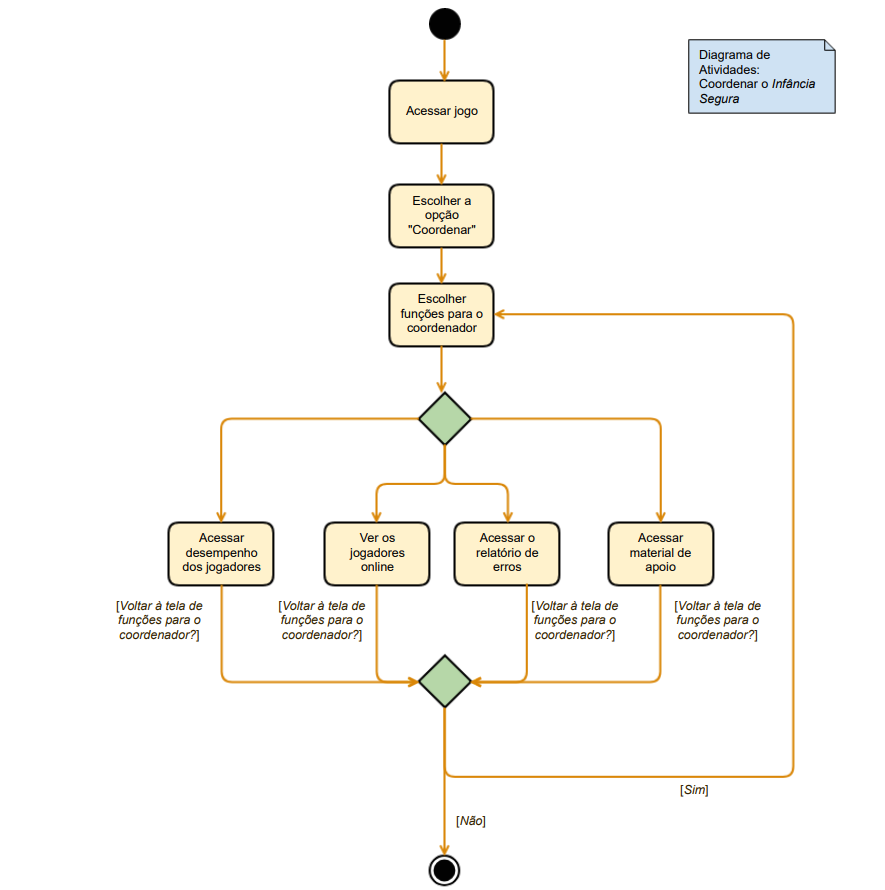
\includegraphics[width=\linewidth]{JogoOriginal/AtividadesCoordenador.png}}
  \caption{Diagrama de Atividades do Educador \citep{diocesano2018jogo}} 
  \label{fig:DiagramaCoordenar}
\end{figure}

O diagrama de atividades do educador apresentado na \cref{fig:DiagramaCoordenar}, demonstra a relação entre as atividades cabíveis ao educador, onde a transição entre as atividades é o resultado direto de suas ações. As três primeiras opções visam  dar um panorama geral acerca dos jogadores, enquanto a quarta opção contém uma lista de endereços (\textit{links}) para páginas na \textit{internet} com materiais didáticos sobre a sexualidade infantil e prevenção da violência sexual infantil. 

A opção \textbf{Desempenhos dos jogadores} comporta uma sub-região da aplicação, na qual o professor precisa especificar uma fase. Ao ser especificada, o professor acessa uma lista nominal de todas as crianças que passaram pela fase em questão e suas respectivas pontuações, além do tempo que permaneceram na fase.

A segunda opção \textbf{Alunos Online no Jogo} leva o professor a uma sala na qual obtém acesso aos nomes das crianças que encontram-se utilizando a aplicação no presente momento e que já tenham informado seus nomes para o sistema. 

A opção \textbf{Relatório de erros dos jogadores} agrega uma outra zona de opções, na qual o professor é convidado a selecionar uma determinada fase do jogo (\cref{fig:ErrosFases}). Quando selecionada, o professor tem acesso a um relatório do nome, da quantidade e dos tipos de erros cometidos pelas crianças na presente fase (\cref{fig:ErrosFase}).

 \begin{figure}[h]
  \centering
  \subfloat[Zona de opções principal]{\frame{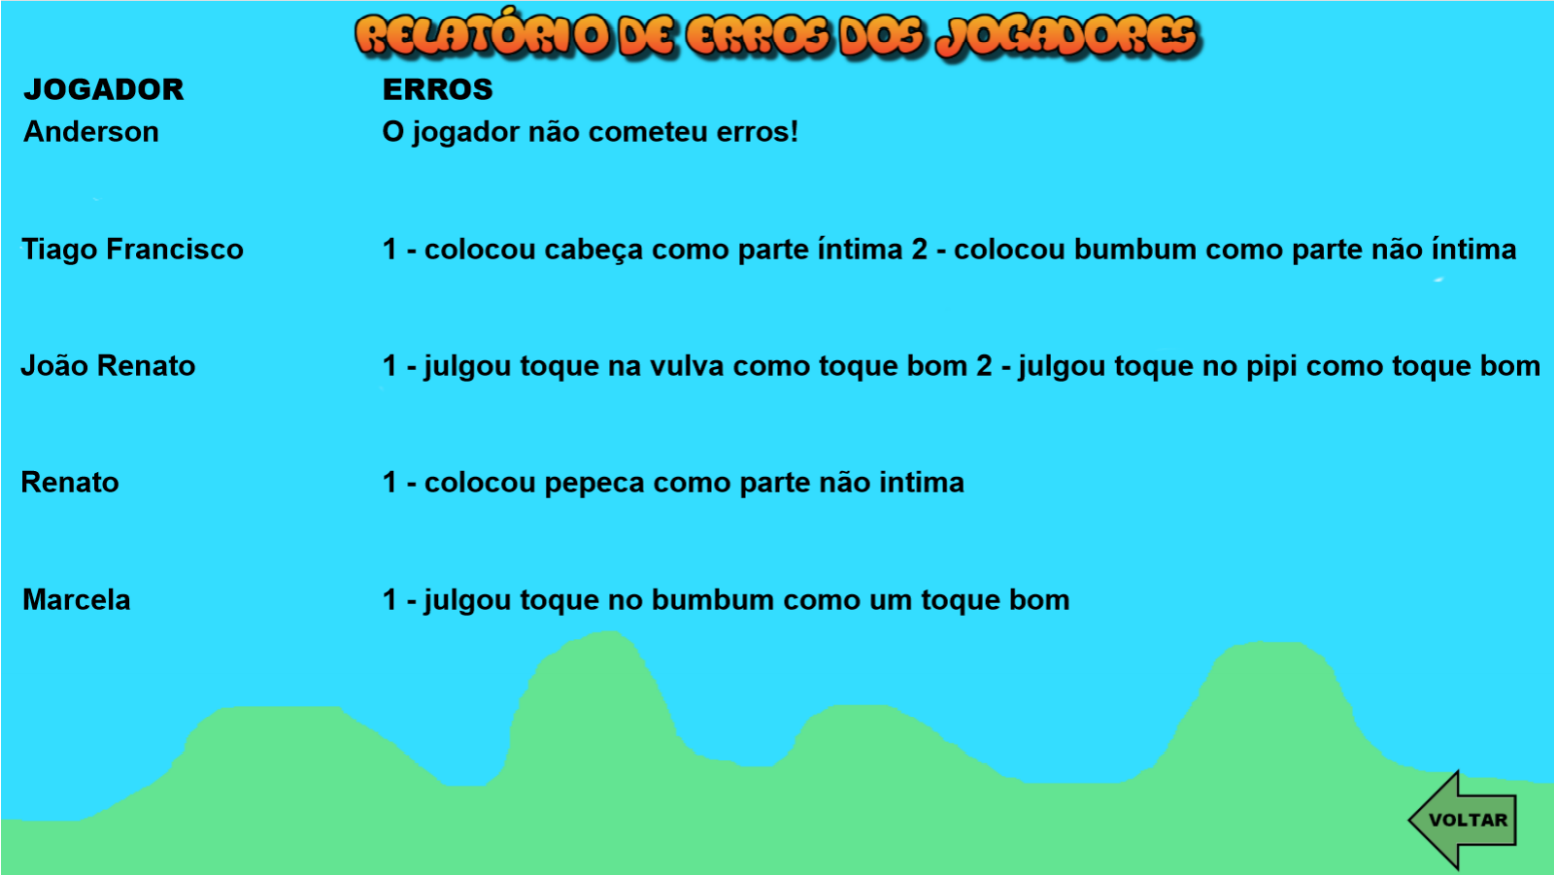
\includegraphics[width=0.49\linewidth]{JogoOriginal/MenuRelatorioErros.png}}\label{fig:ErrosFases}}\hspace{0.1mm}
  \subfloat[Erros registrado em uma fase]{\frame{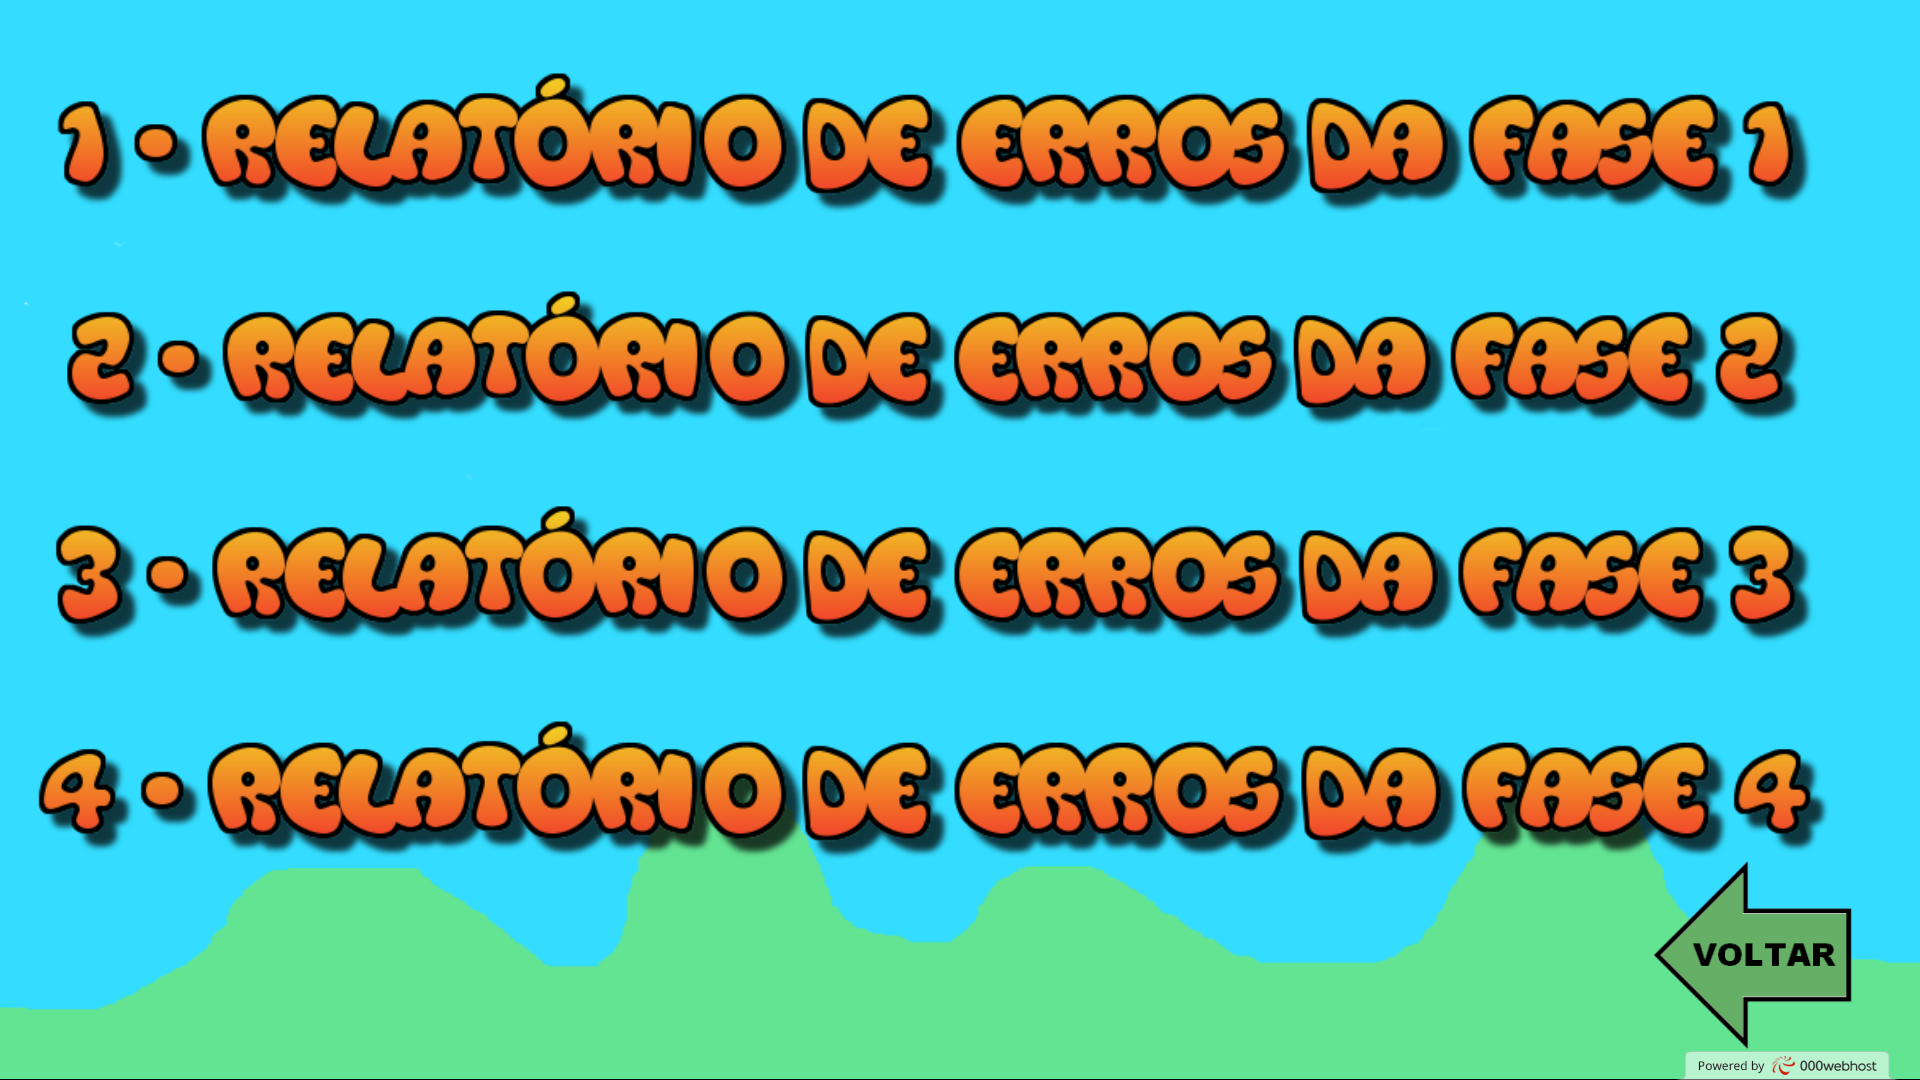
\includegraphics[width=0.49\linewidth]{JogoOriginal/RelatorioErros.png}}\label{fig:ErrosFase}}
  \caption{Relatório de Erros}
  \label{fig:RelatorioErros}
\end{figure}

Por fim, a opção \textbf{Links importantes}, agrega uma lista de endereços (\textit{links}) para páginas na \textit{internet} com materiais didáticos sobre a sexualidade infantil e prevenção da violência sexual infantil. Entre esses materiais, há \textit{links} para vídeos explicativos, apostilas, manuais, entre outros materiais na temática em questão.


\section{Análise do Jogo}\label{secao:EstudoArte}

Jogos são utilizados como instrumento recreativo ou como instrumento educacional há anos \citep{batista2007estudo, tarouco2004jogos}. Em virtude disso, surgiram inúmeros materiais e manuais com recomendações para o desenvolvimento e criação de jogos \citep{arruda2014fundamentos, alves2019unity}. Nesse sentido, o jogo \textbf{Infânci Segura} foi confrontado pela presente pesquisa e analisado sob uma visão técnica no que diz respeito ao cumprimento de certas normas presentes na literatura. 

\pagebreak

De início, encontraram-se discrepâncias entre a literatura e o jogo \textbf{Infância Segura}, além de falhas de segurança. Destaca-se nesse sentido, que não há separação segura entre as atividades do jogador e as atividades do educador. Uma criança, ou qualquer terceiro, poderia acessar o jogo e adentrar na zona do educador sem demais empecilhos, a ponto de ter total acesso as informações dos jogadores. Uma requisição de senha, seria suficiente para dificultar quaisquer ações do gênero. %Todavia, isso ainda não resolveria a quebra de requisitos básicos de percepção \citep{mantau2013analise}.

O jogo \textbf{Infância Segura}, no que diz respeito aos requisitos de percepção, comporta atividades que não deveriam ser acessadas pelo jogador. Nesse quesito, a literatura diz que a interface de um sistema não deve conter informações desnecessárias ou que não serão utilizadas \citep{mantau2013analise}. Para corrigir esse quesito, seria necessário dividir o jogo \textbf{Infância Segura} em duas aplicações: uma destinada somente aos jogadores, contendo o jogo em si; e outra destinada aos professores, contendo toda a plataforma de apoio e coordenação.

O jogo também desconsidera requisitos de flexibilidade, fazendo o jogador ter que executar as fases (\cref{subsecao:Jogar}) na mesma ordem. Em termos gerais, a literatura diz que um sistema deve ser flexível, liberando o jogador da necessidade de seguir linearmente o conteúdo e as atividades propostas pelo jogo \citep{mano2005interfaces}.

A literatura revelou ainda alguns descumprimentos técnicos e outros pedagógicos cometidos no jogo original. Dentre os descumprimentos pedagógicos destaca-se o uso de ordens negativas em algumas fases, ordens as quais, poderiam induzir as crianças a fazerem de fato as atitudes classificadas como proibidas \citep{florentino2015possiveis}. Dos descumprimentos técnicos, enfatiza-se a ausência de padronização no sistema \citep{nielsen1993usability}, sendo um exemplo: a utilização de textos em caixa alta em algumas telas do sistema e em outra não (textos usados no mesmo contexto), vide a \cref{fig:JogoOriginal} e a \cref{fig:PrincipalCoordenar}, ambos uma zona de opções, porém apresentadas de formas distintas.

A revisão realizada no presente artigo revelou dez descumprimentos entre o jogo analisado e as bases da literatura para desenvolvimento e criação de jogos. Como resultado, constatou-se a necessidade da remodelagem do jogo de modo a alinhá-lo com orientações técnicas e pedagógicas, tal necessidade se acentua ainda mais em virtude da sensibilidade da temática do jogo revisado.

O tempo gasto no desenvolvimento de um \textit{software} está, em algum nível, associado com a qualidade do mesmo. Desta forma, manifesta-se a necessidade de busca por estratégias de menor tempo que mantenham (ou aumentem) a qualidade do produto desenvolvido. O jogo \textbf{Infânci Segura} entrelaça as atividades do jogador e as atividades do educador em um único sistema, o que descumpre requisitos básicos de percepção \citep{mantau2013analise}. Deste modo, o desenvolvimento de uma nova versão do jogo \textbf{Infânci Segura} com as atividades do jogador e do educador separadas desde o princípio apresenta-se menos custosa.

\pagebreak

\section{Novo Jogo}\label{secao:InfanciaSegura2.0}

Como proposta desse trabalho, uma nova versão do jogo \textbf{Infância Segura} foi desenvolvida. Seu desenvolvimento é fundamentado nas recomendações de especialistas e manuais sobre a criação e desenvolvimento de jogos, vide os apontamentos realizados na \cref{secao:EstudoArte}. A nova versão surge sob um ponto de vista mais técnico, porém sem deixar de lado a essência do jogo original. Os ensinamentos e conteúdos ministrados foram preservados, uma vez constatada a concordância entre eles e `orientações técnicas internacionais de educação em sexualidade' \citep{women2018international}.

O jogo foi desenvolvido no motor de jogos \mbox{\textit{Construct 2}}\footnote{O Construct 2 é um motor de jogos para o desenvolvimento de jogos digitais multiplataforma em 2D baseados em HTML 5, sendo distribuído pela Scirra Ltda (Disponível em: \underline{\url{https://www.scirra.com/store/construct-2}})}, com uma separação clara entre a aplicação voltada ao jogador e a aplicação voltada ao educador. Em outras palavras, é proposto por esse trabalho um jogo sério para a prevenção da violência sexual infantil, o qual é apresentado na \cref{subsecao:JogoEducacional} e uma plataforma de apoio aos professores, apresentada na \cref{subsecao:PlataformaApoio}. %Os dois \textit{softwares} desenvolvidos estão conectados por um banco de dados, sendo cada versão independente entre si. 


\subsection{Jogo Sério}\label{subsecao:JogoEducacional}

A presente seção destaca os principais pontos da aplicação desenvolvida voltada para o público infantil. Na corrente versão os registros básicos do usuário são armazenados no aparelho onde o jogo estiver sendo executado (\textit{Local Storage}). Desta maneira, todas as conquistas, atividades e ações realizadas pelo jogador são recarregadas sempre que o jogador reacessar o jogo, removendo assim a necessidade de uma autenticação manual a cada reacesso. 

Para uma criança obter acesso ao jogo, é necessário antes concordar com os termos de uso, informar seu nome, informar seu gênero, escolher um \textit{token} de identificação, adentrar em uma turma, escolher um personagem, e por fim selecionar um amigo virtual. 

Uma maior quantidade de informações é requisitada aos jogadores (em relação a versão original) a fim de tornar o jogo mais seguro. Somado a isso, destaca-se que ao contrário da progressão linear de fases do jogo original (\cref{subsecao:Jogar}), a nova versão assume o caráter de um jogo no estilo \textit{Role-Playing Game} (RPG), os quais englobam jogos de mundo aberto, onde o jogador pode andar pelo cenário e interagir com outros personagens do jogo \citep{morais2018desenvolvimento}.

A conversão do jogo linear original em um RPG foi realizada principalmente para trazer mais liberdade e flexibilidade ao jogador. Além disso, tal gênero de jogo permite um maior desenvolvimento de habilidades como atenção, concentração, representação, criatividade e socialização \citep{pessini2015ferramenta}. Salientando nesse sentido que não há a socialização entre jogadores no novo jogo proposto.  

Os jogos no estilo RPG possuem vantagens para uso no contexto educacional. Por serem jogos de mundo aberto, os jogadores são auxiliados (educados), seja com um tutorial, ou seja com uma narrativa para contextualiza-los no mundo, trazendo assim, amparo aos jogadores. Como base neste contexto, a nova versão do jogo \textbf{Infância Segura} traz um  amigo virtual (tutor), que deve ser selecionado obrigatoriamente pelo jogador, para que ele possa adentar no jogo. 

 \begin{figure}[h]
  \centering
  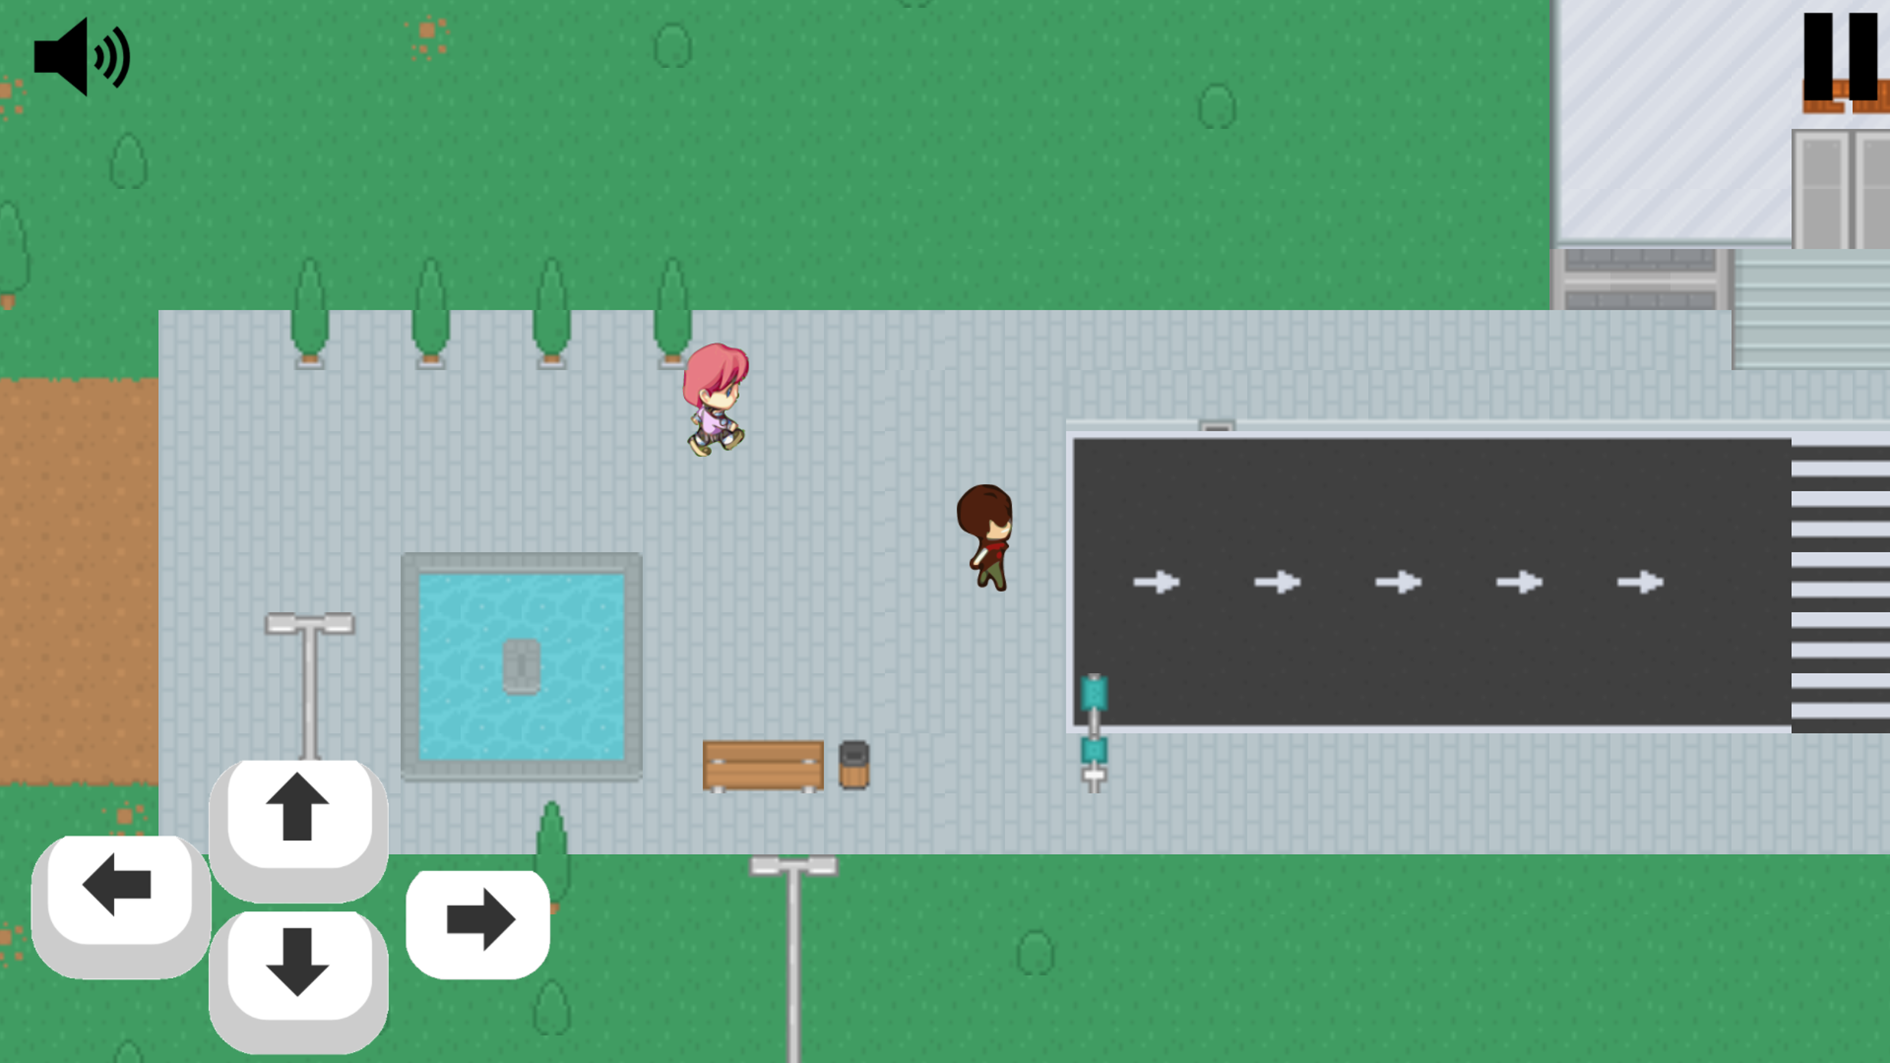
\includegraphics[width=\linewidth]{NovoJogo/Mundo.png}
  \caption{Mundo Virtual do Novo Jogo}
  \label{fig:MundoNovoJogo}
\end{figure}


A \cref{fig:MundoNovoJogo} mostra uma fração do mundo virtual do jogo desenvolvido pela presente pesquisa. O personagem ao centro representa o personagem selecionado pela criança, na qual suas ações de locomoção podem ser executadas pelas setas do teclado, ou pelas setas situadas no canto inferior esquerdo da tela do aparelho. O outro personagem à noroeste do personagem central é o amigo virtual selecionado pelo jogador, o qual funciona como um tutor que explica sobre o funcionamento e as ações permitidas no jogo. Cabe destacar que o amigo virtual também é utilizado para suportar a dinâmica do herói mudo ou protagonista silencioso \citep{domsch2017dialogue}. 

A dinâmica do herói mudo permite uma imersão maior ao jogador, pois permite uma conexão mais forte entre personagem e jogador, uma vez que não há o risco do personagem se utilizar de palavras ou de elementos contextuais que o jogador desconheça \citep{domsch2017dialogue}. Nesse sentido, as perguntas são transferidas para um personagem que o jogador não possui controle (o amigo virtual), com o intuito de evitar assim, uma disrupção da interligação entre personagem e jogador.

O amigo virtual interage com o jogador por intermédio de texto e áudio. No momento que o jogador adentra no mundo do jogo pela primeira vez, o amigo virtual introduz os ambientes disponíveis para exploração dando uma breve descrição dos conteúdos neles ministrados, como pode ser observado na \cref{fig:AmbientesNovoJogo}. Salienta-se nesse sentido, que não apenas o amigo virtual encontra-se dublado, mas também todos os textos que são apresentados eventualmente ao jogador, facilitando assim o entendimento da narrativa do jogo por parte das crianças que se encontram em processo de alfabetização.

\newpage

 \begin{figure}[h]
  \centering
  \subfloat[Apresentação do Hospital]{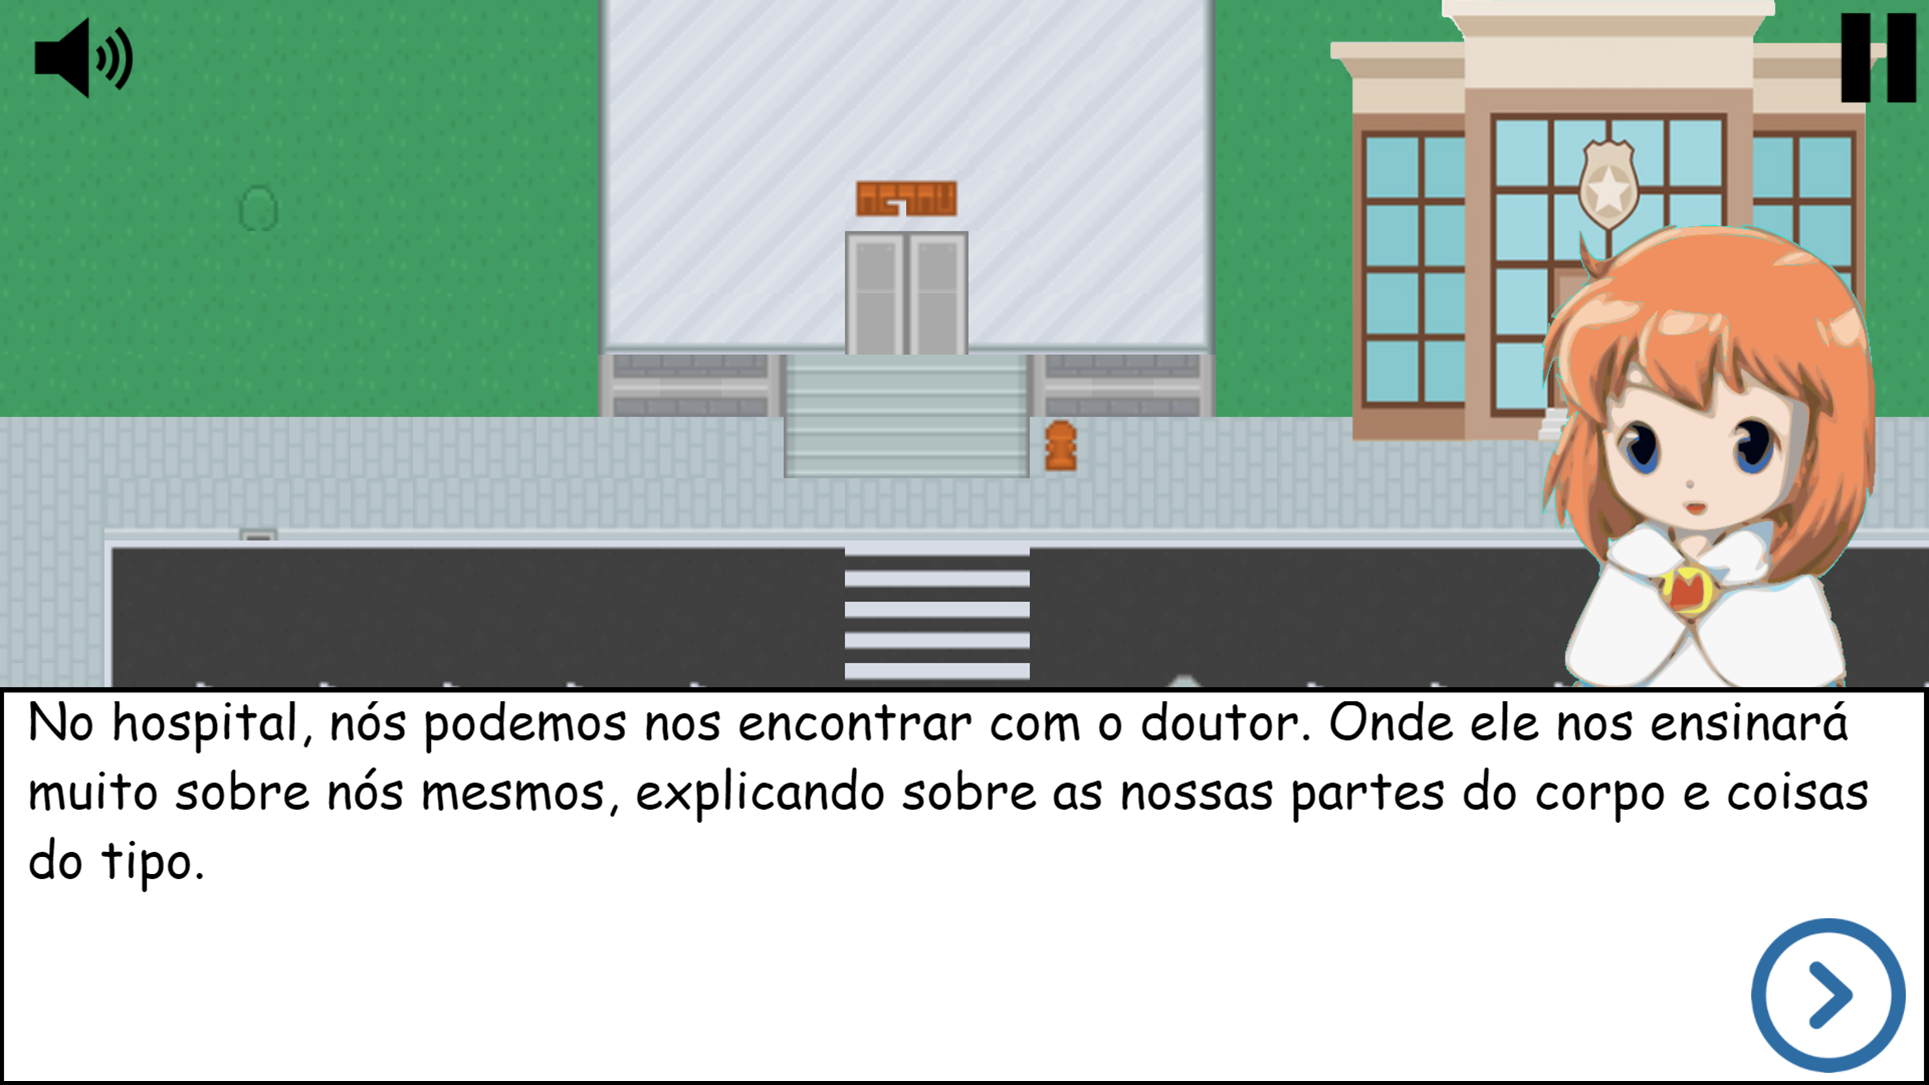
\includegraphics[width=0.49\linewidth]{NovoJogo/Fase1.png}\label{fig:AmbientesNovoJogo1}}\hspace{0.1mm}
  \subfloat[Apresentação da Delegacia]{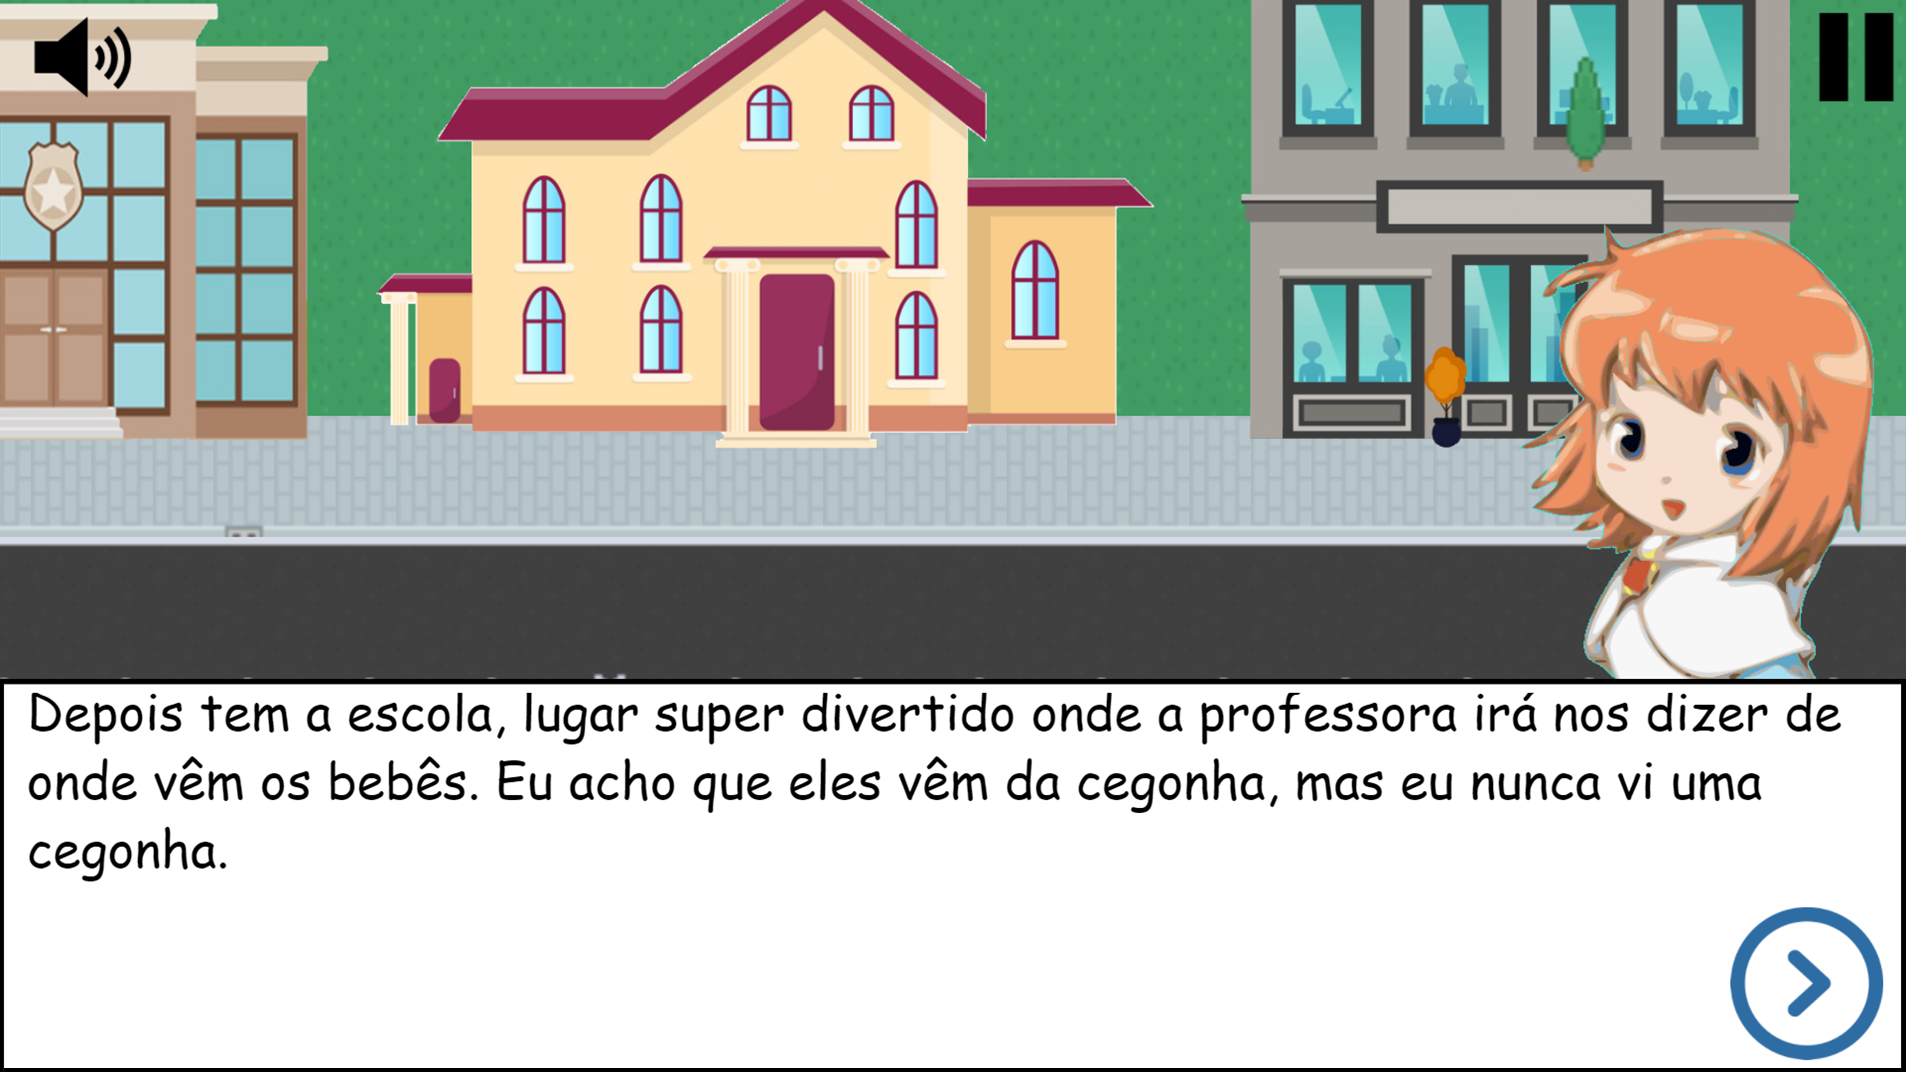
\includegraphics[width=0.49\linewidth]{NovoJogo/Fase2.png}\label{fig:AmbientesNovoJogo2}}
  \hfill \vspace{- 0.3 cm}
  \subfloat[Apresentação da Escola]{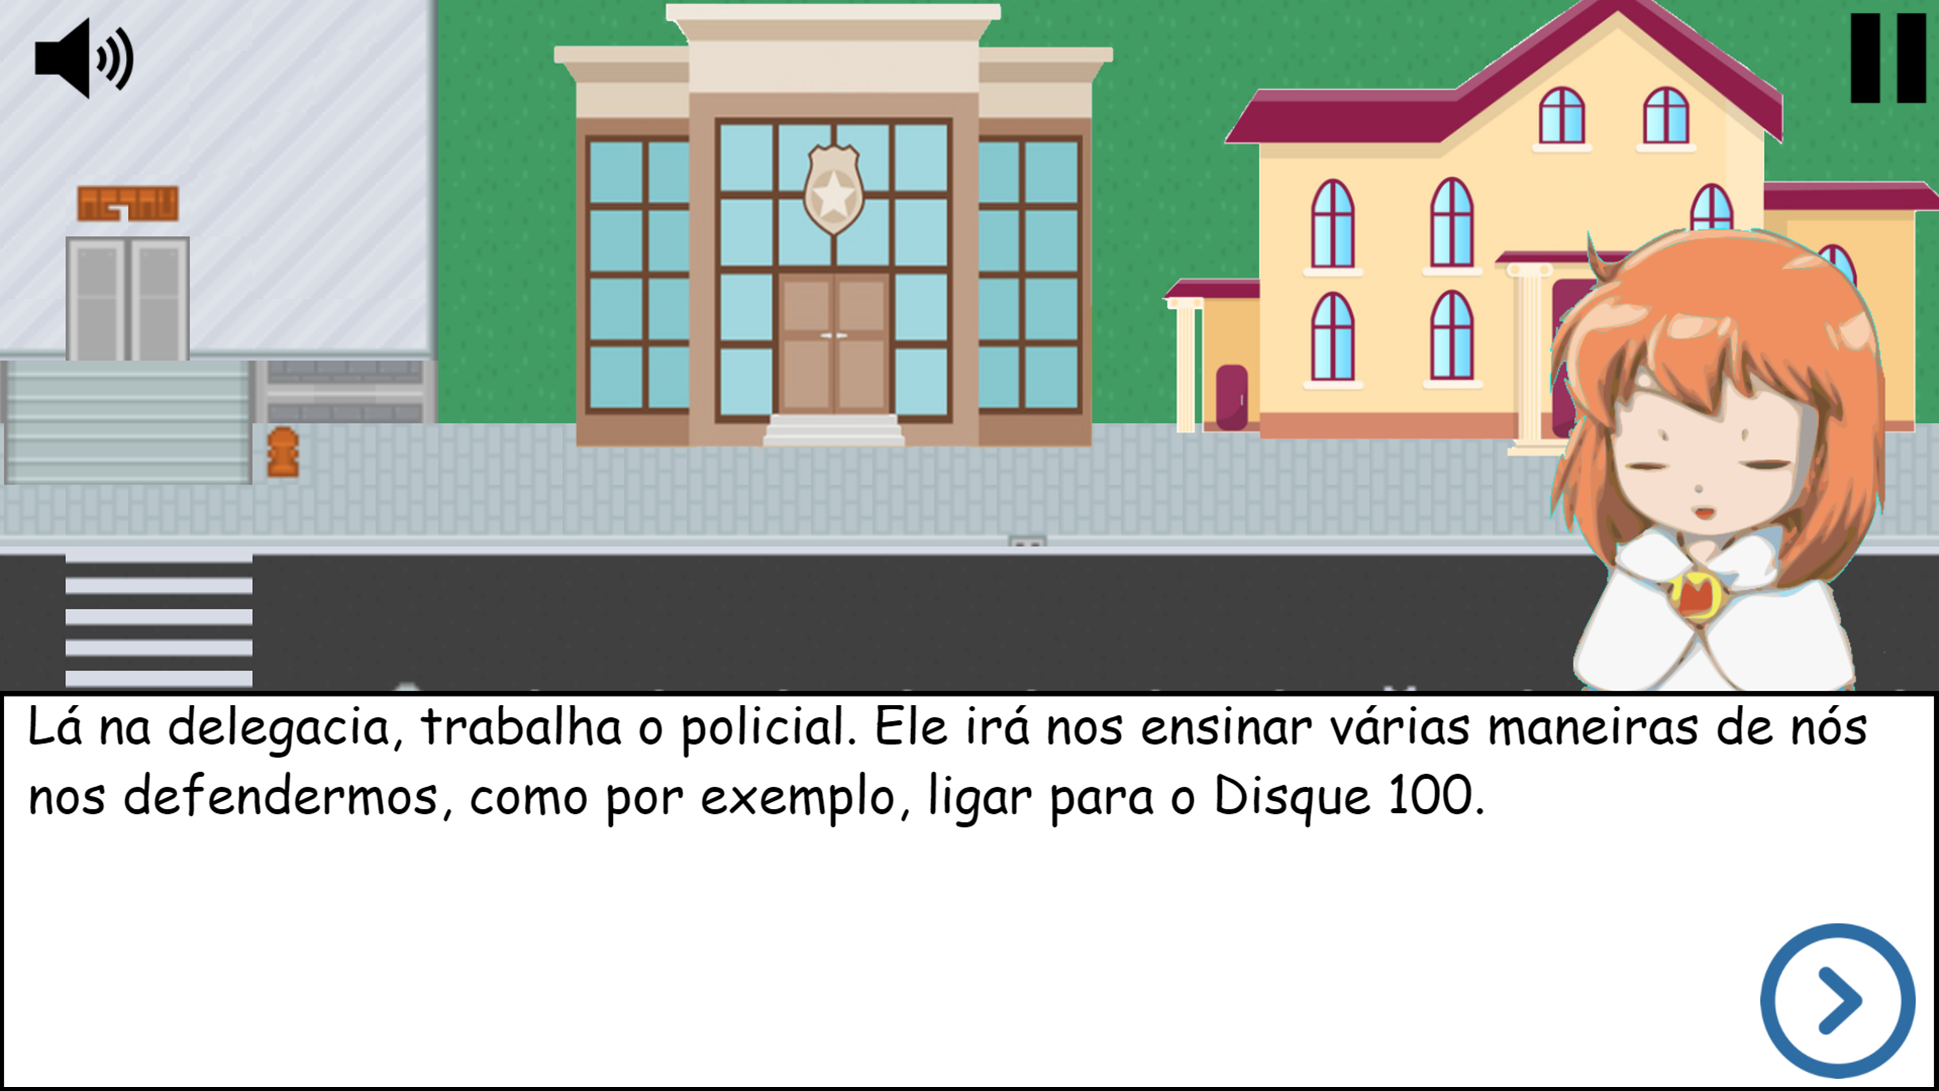
\includegraphics[width=0.49\linewidth]{NovoJogo/Fase3.png}\label{fig:AmbientesNovoJogo3}}\hspace{0.1mm}
  \subfloat[Apresentação da \textit{Lan House}]{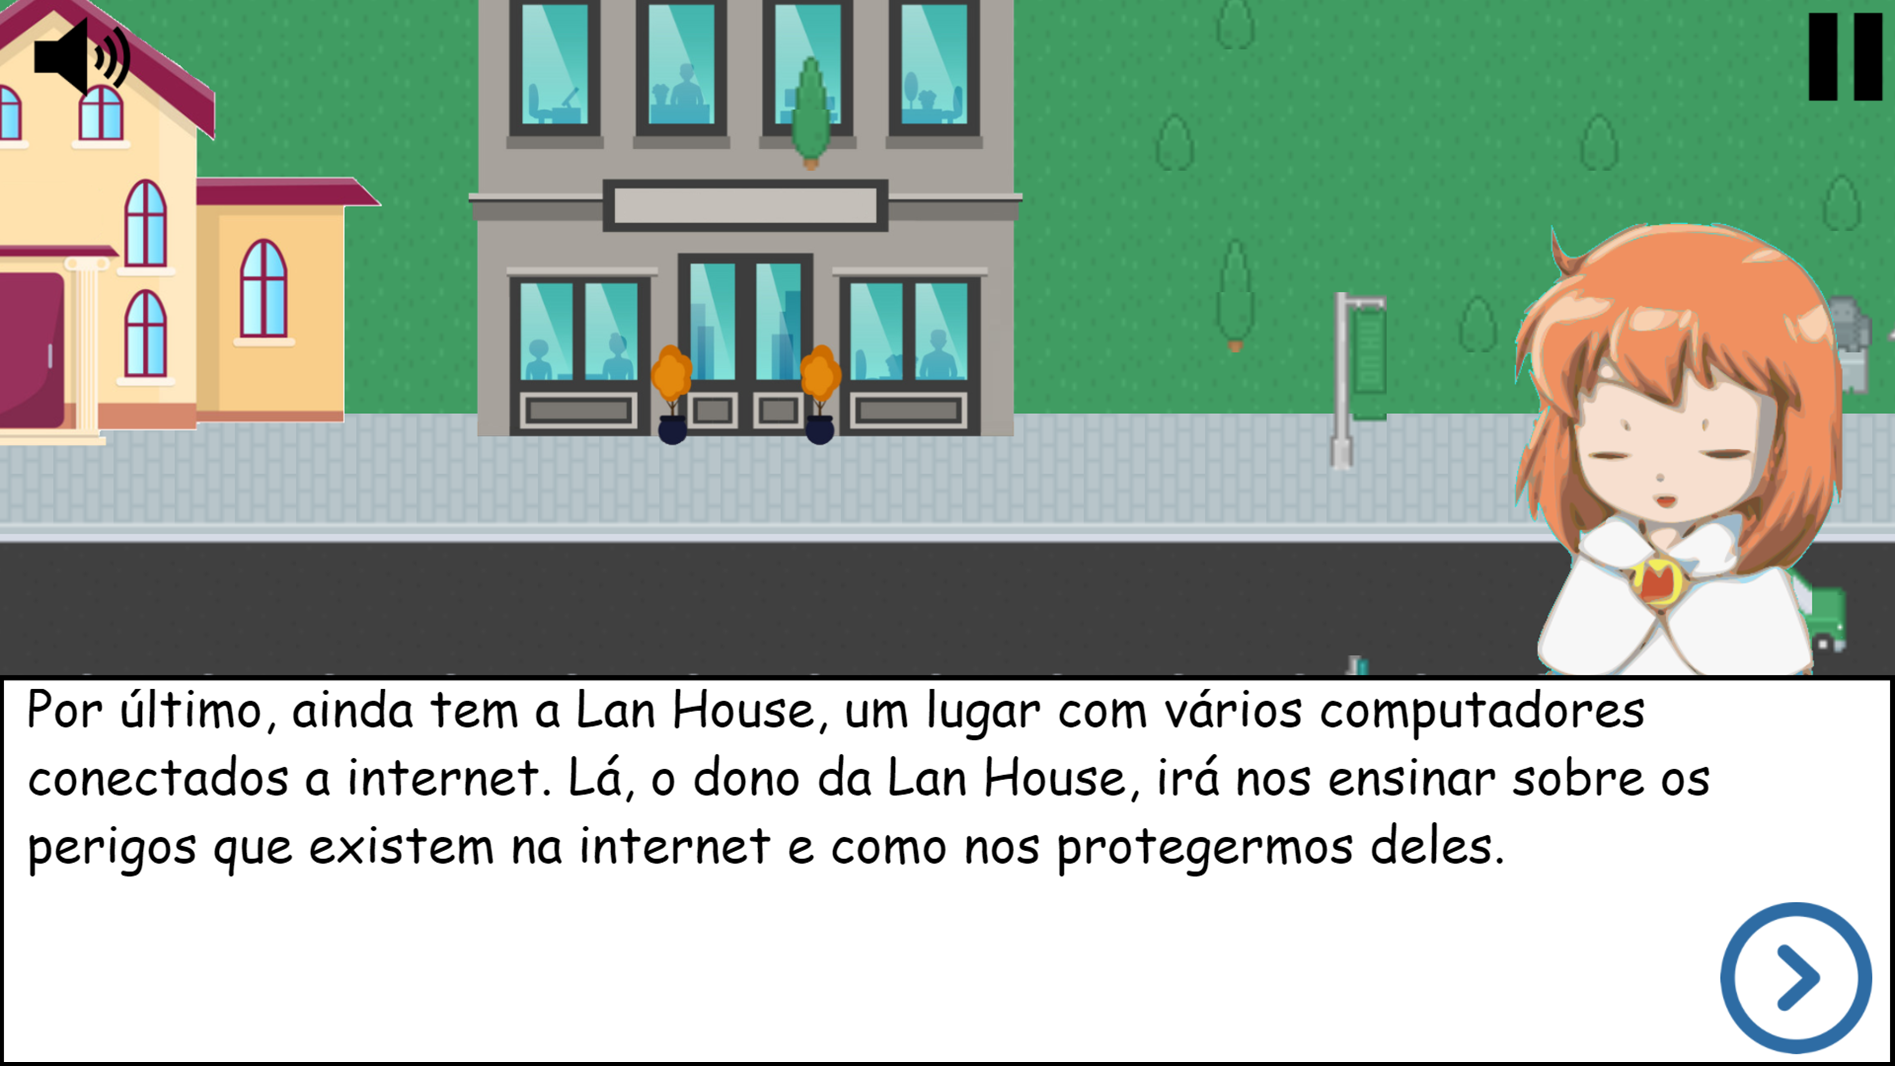
\includegraphics[width=0.49\linewidth]{NovoJogo/Fase4.png}\label{fig:AmbientesNovoJogo4}}
  \caption{Telas dos Cenários do Novo Jogo}
  \label{fig:AmbientesNovoJogo}
\end{figure}

\vspace{- 0.4 cm}

As telas da \cref{fig:AmbientesNovoJogo} apresentam os quatro cenários onde os conteúdos são ministrados. Na \cref{fig:AmbientesNovoJogo1}, o amigo virtual introduz o Hospital, já na \cref{fig:AmbientesNovoJogo2} é apresentada a Delegacia, na \cref{fig:AmbientesNovoJogo3} a Escola e na \cref{fig:AmbientesNovoJogo4} a \textit{Lan House}. Cada local é apresentado brevemente, dando ao jogador uma vaga noção sobre as lições que são abordadas nos respectivos ambientes. Ao fim, o usuário é ensinado sobre a forma de como transitar entre os locais.

O jogo permite que o jogador explore o mundo virtual dentro de seus limites. Nas extremidades do mundo há uma barreira que impede o jogador de sair para fora do mapa do jogo. Todavia, dentro deste limite o jogador é livre para intercambiar entre os ambientes da maneira que melhor lhe convir. No Hospital por exemplo, o personagem de um médico ensina o jogador sobre o nome das partes do corpo, sobre as partes íntimas e sobre os `toques bons' e `toques ruins'. A primeira lição lecionada (apresentação das partes do corpo), é apresentada em maiores detalhes na \cref{fig:Hospital}.

\vspace{- 0.3 cm}

 \begin{figure}[h]
  \centering
  \frame{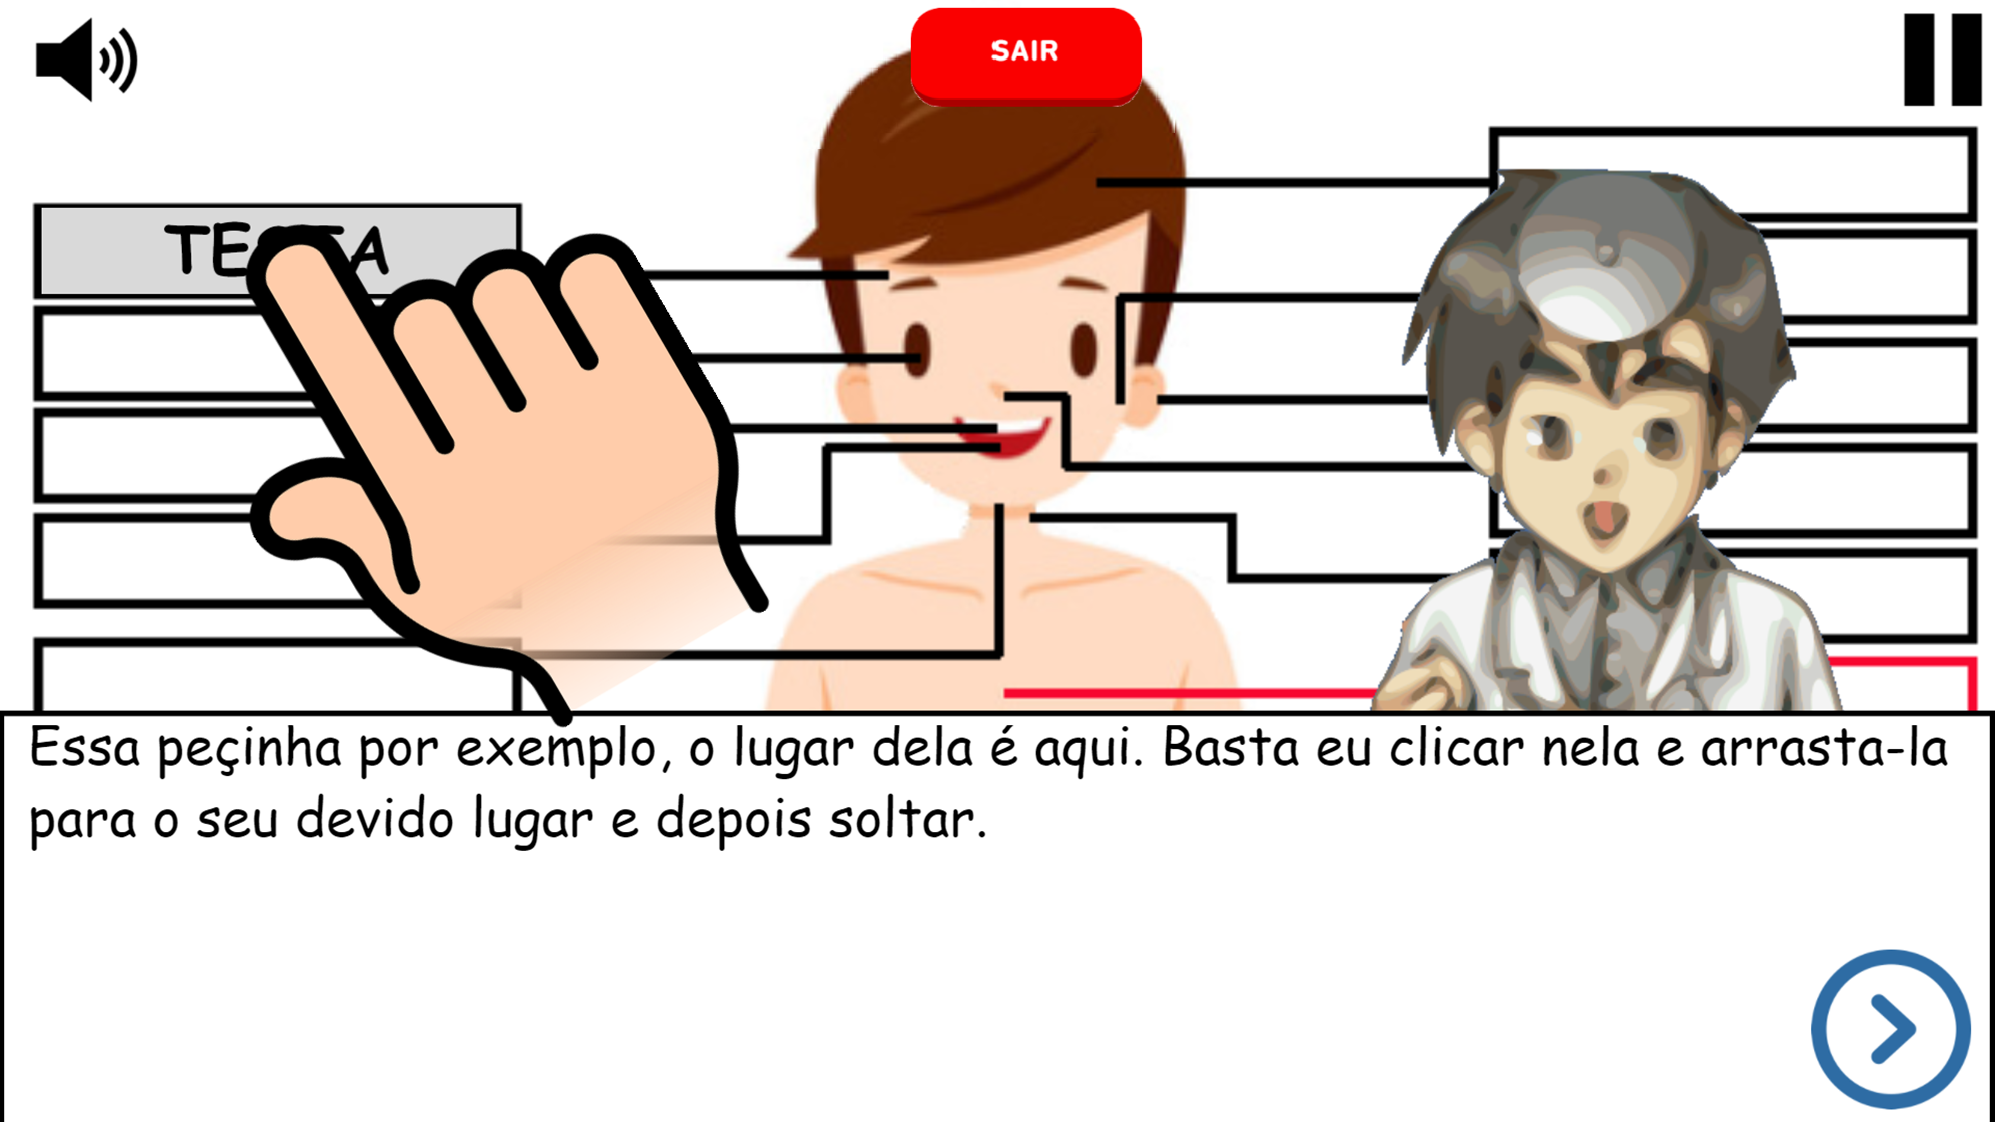
\includegraphics[width=\linewidth]{NovoJogo/JogoFase1.png}}
  \caption{Fase 1 - Hospital do Novo Jogo}
  \label{fig:Hospital}
\end{figure} 

\vspace{- 0.4 cm}

A \cref{fig:Hospital} ilustra a fase do Hospital. A dinâmica de jogo na fase do Hospital é no estilo \textit{Drag-and-drop}, onde a criança precisa arrastar e soltar as peças para seus respectivos lugares, no presente exemplo: arrastar os nomes das partes do corpo para suas devidas regiões em um mural do corpo humano sem as legendas. Salienta-se que até o presente momento, apenas a fase do Hospital encontra-se desenvolvida.


\subsection{Plataforma de Apoio Pedagógica}\label{subsecao:PlataformaApoio}

A atual seção apresenta os principais pontos da aplicação desenvolvida para apoio pedagógico. Para obter acesso é necessário o preenchimento de seis campos obrigatórios, sendo eles: Nome, Email, Senha, Escola, Cidade, Estado. Uma vez preenchidos, o professor adentra na plataforma. Todas as informações preenchidas são enviadas para um banco de dados e armazenadas no próprio dispositivo (\textit{Local Storage}), desta forma, o professor não precisa se autenticar toda vez que for acessar a ferramenta. 


 \begin{figure}[h]
  \centering
  \subfloat[Tela Principal]{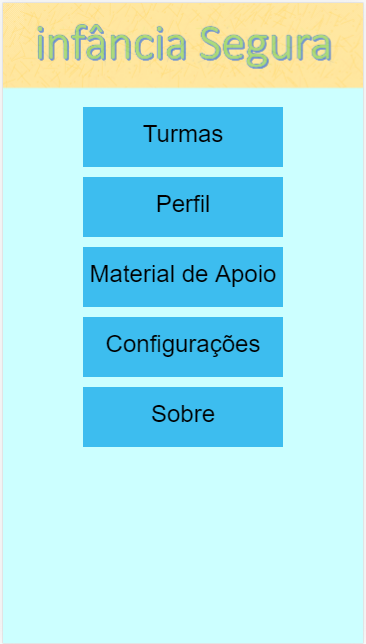
\includegraphics[width=0.24\linewidth]{PlataformaApoio/CoordenarInicio.png}}\label{fig:PlataformaApoio1}
  \subfloat[Configurações]{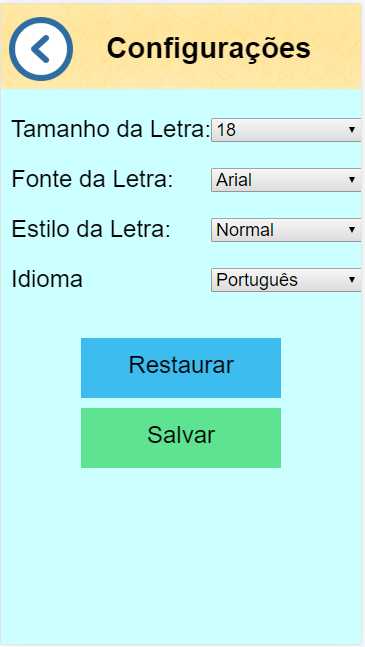
\includegraphics[width=0.24\linewidth]{PlataformaApoio/CoordenarConfiguracoes.png}\label{fig:PlataformaApoio2}}
  \subfloat[Tela Materiais]{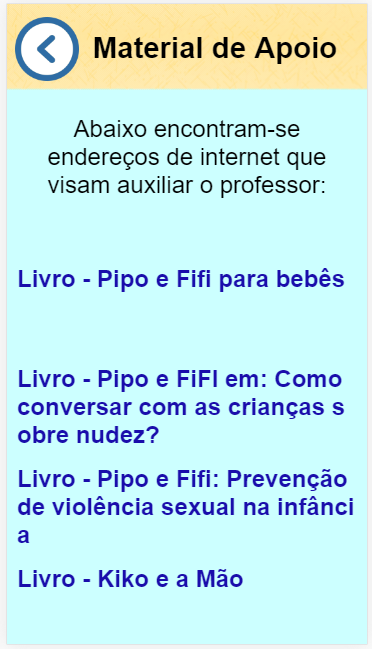
\includegraphics[width=0.24\linewidth]{PlataformaApoio/CoordenarMaterialApoio.png}\label{fig:PlataformaApoio3}}
  \subfloat[Tela do Perfil]{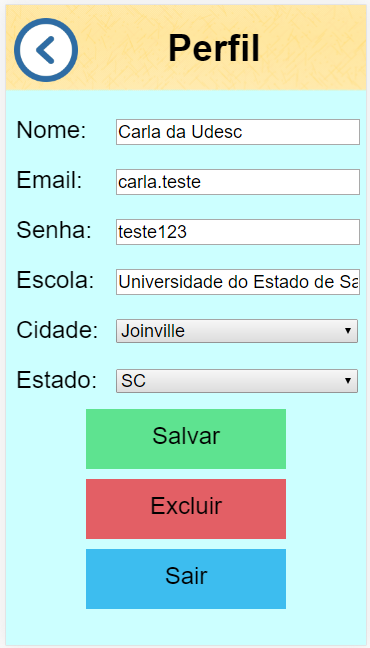
\includegraphics[width=0.24\linewidth]{PlataformaApoio/CoordenarPerfil.png}\label{fig:PlataformaApoio4}}
  \hfill
  \subfloat[Tela Turmas]{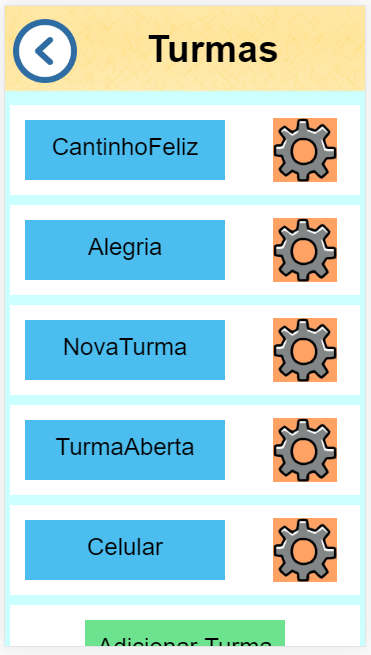
\includegraphics[width=0.24\linewidth]{PlataformaApoio/CoordenarTurmas.png}\label{fig:PlataformaApoio5}}
  \subfloat[Tela de Ajustes]{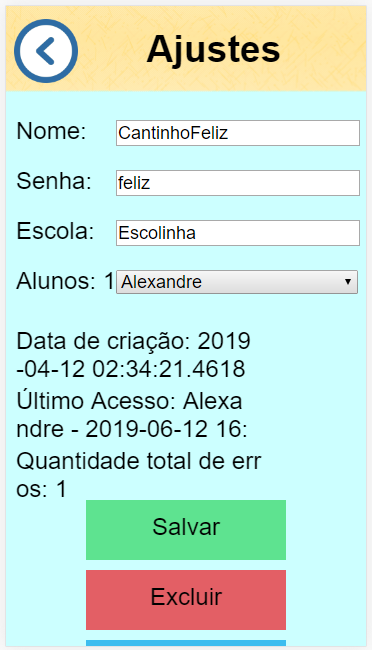
\includegraphics[width=0.24\linewidth]{PlataformaApoio/CoordenarAjustes.png}\label{fig:PlataformaApoio6}}
  \subfloat[Tela da Turma]{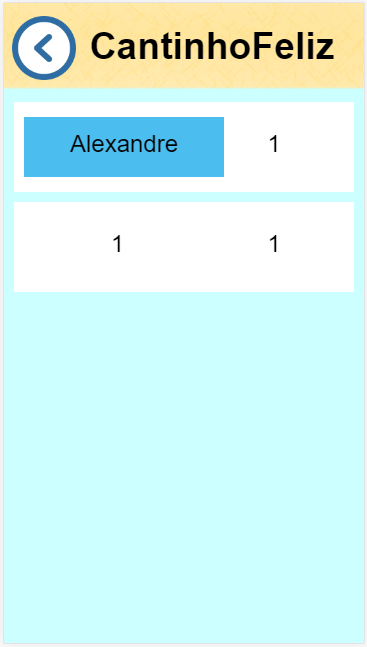
\includegraphics[width=0.24\linewidth]{PlataformaApoio/CoordenarTurma.png}\label{fig:PlataformaApoio7}}
  \subfloat[Tela do Aluno]{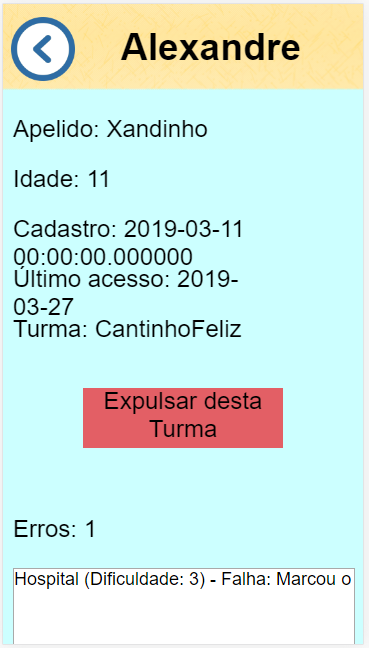
\includegraphics[width=0.24\linewidth]{PlataformaApoio/CoordenarAluno.png}\label{fig:PlataformaApoio8}}
  \caption{Telas da Plataforma de Apoio Pedagógica}
  \label{fig:PlataformaApoio}
\end{figure} 


A \cref{fig:PlataformaApoio} mostra as telas do sistema de apoio ao professor sendo apresentadas na versão \textit{mobile}. Nesse sentido, cabe ressaltar que tanto o jogo (\cref{subsecao:JogoEducacional}), quanto a apresente plataforma de apoio são \textit{softwares} responsivos, se adaptando as proporções do ecrã do usuário (diferentemente do jogo original). A \cref{fig:PlataformaApoio1} apresenta uma zona de opções. Tal zona é carregada no momento da autenticação do professor, permitindo-o alcançar todas as demais telas do sistema. 

A opção \textbf{Turma}, da zona de opções, apresenta uma nova tela com todas as turmas que foram criadas para serem coordenadas. A seleção do \textbf{Perfil}, leva o usuário a uma nova tela, onde lhe é permitido a visualização e edição de suas informações. O botão \textbf{Material de Apoio} carrega uma lista de endereços em uma nova tela na aplicação. A opção \textbf{Configurações} redireciona o usuário a um leiaute com capacidades de configuração e personalização. A opção \textbf{Sobre}, quando pressionada, carrega uma breve descrição sobre o \textit{software}.

No sistema em questão, o coordenador possui total liberdade para criar e gerenciar suas turmas. Uma vez que uma turma tenha sido cadastrada no sistema, as crianças podem se inscrever na turma. Ao selecionar uma turma, o professor tem acesso a lista dos alunos cadastrados naquela turma, e ao selecionar um aluno, o professor é confrontado com algumas informações geradas pelo aluno selecionado durante sua jogatina, como: data de cadastro, quantidade de erros, quantidade de acertos, descrição dos erros e acertos (\cref{fig:PlataformaApoio8}).

Salienta-se que o \textit{software} em questão assume algumas características de um \textit{Learning Analytics} (LA) servindo como um instrumento auxiliador para a identificação e análise dos dados estudantis \citep{prante2018professor}. O sistema coleta, mede, analisa e relata os dados e seus contextos com objetivo de otimizar a gestão pedagógica.

\section{Experimentos}\label{secao:Experimentos}

Avaliações e testes de usuários são etapas fundamentais no desenvolvimento de \textit{software}. No campo dos jogos educacionais é importante realizar avaliações para assegurar que eles trazem benefícios a fim de justificar sua utilização na sala de aula \citep{campos1996dez}. Dentre os métodos avaliativos encontra-se o modelo de avaliação \textit{Model for the Evaluation of Educational Games} (MEEGA) desenvolvido por \cite{savi2011avaliaccao}.

O modelo teórico e o questionário do modelo MEEGA são usados como base pelo presente trabalho. %, visando a análise dos jogos de maneira a fornecer resultados promissores de forma rápida e prática \citep{savi2011avaliaccao}. 
Apenas os \textit{softwares} voltados ao público infantil foram avaliados (tanto o jogo original, quanto a nova versão desenvolvida pela presente pesquisa). Nesse sentido cabe salientar que o questionário do modelo MEEGA foi adaptado seguindo suas próprias recomendações de adaptação \citep{savi2011model}. O questionário foi modificado buscando deixá-lo mais adequado e simples para crianças.%, porém sem perder sua essência primordial.

O formato de medição utilizado no questionário é baseado em itens Likert \citep{likert1932technique}. Cada item do questionário serve para quantificar os sentimentos dos participantes em relação aos jogos analisados, onde os participantes são confrontados com indagações acerca dos jogos de modo a indicarem sua opinião, e também informarem o grau de discordância ou concordância em uma escala valorada entre -2 e +2. Considerando a natureza infantil dos participantes, optou-se por uma escala gráfica, ao invés de uma escala numérica.


%No dia 30 de maio de 2019 (quinta-feira) às 19:30 o processo avaliativo deu início.O experimento realizado durou cerca de duas horas, terminando às 21:30, com resultados promissores. 
O processo avaliativo foi realizado com duas crianças. Um menino de 6 anos (em fase de alfabetização) e uma menina de 12 anos.

\newpage

A seleção de um número reduzido de usuários (duas crianças) visa evitar expor uma maior quantidade de crianças a qualquer impacto negativo que um dos jogos pudesse causar. Desta forma, é possível supervisionar os menores durante todo o experimento, garantindo assim sua saúde e bem estar. Salienta-se ainda que um dos responsáveis das crianças esteve presente durante a execução dos testes.%, retirando assim, a necessidade de termos de consentimento pela atual pesquisa, uma vez que a presença de um dos responsáveis já configura legalmente uma autorização tácita. 

Os participantes selecionados, até o momento do processo avaliativo, não haviam tido nenhum contato prévio com o presente autor, descartando desta forma, quaisquer tendências ou inclinações durante a avaliação; com os jogos sendo submetidos as crianças de maneira cega (teste cego), sem as mesma saberem seus devidos arquitetos e com os jogos sendo submetidos de forma alternada entre os menores. Cada participante foi submetido ao mesmo questionário duas vezes, cada qual, associado a uma das versões do jogo \textbf{Infância Segura}.

No momento do processo avaliativo, o novo jogo não se encontrava finalizado. Deste modo, informa-se que apenas a \textbf{fase 1} e a \textbf{fase 2} do jogo original (\cref{subsecao:Jogar}) foram submetidas aos participantes durante a avaliação, pois apenas estas fases encontravam-se mapeadas no novo jogo (\cref{subsecao:JogoEducacional}).

O experimento em questão foi realizado com o intuito de averiguar os verdadeiros impactos no cumprimento das bases da literatura sobre o desenvolvimento e criação de jogos. De um lado do experimento, o jogo original se apresentava com seus descumprimentos da literatura (\cref{secao:EstudoArte}); do outro lado do experimento, o novo jogo se apresentava com sua suposta correção destes descumprimentos. Destaca-se que a quantidade reduzida de participantes ajuda apenas na identificação de grandes discrepâncias nos resultados dos jogos, pois o desvio padrão torna-se grande em pequenas amostras.

%O teste piloto realizado serve de precaução para um melhor alinhamento no desenvolvimento atual do jogo \textbf{Infância Segura 2.0} e uma melhor preparação para um futuro experimento devidamente aprovado pelo comitê de ética e com um maior número de participantes.


\section{Resultados}\label{secao:Resultados}

Os dados gerados pela presente pesquisa foram compilados em dois gráficos. Dentre os dados colhidos sobre o jogos avaliados estão informações relacionadas com a \textbf{motivação} (\cref{fig:Motivacao}) e a \textbf{experiência dos usuários} (\cref{fig:ExperienciaUsuario}). A \textbf{motivação} comunica a opinião dos jogadores em relação ao interesse nos conteúdos ministrados e na aparência do jogo. Já a \textbf{experiência dos usuários} quantifica a posição dos jogadores em relação as dinâmicas do jogo e sua imersão no mundo digital.

\newpage

\begin{figure*}[ht]
  \centering
  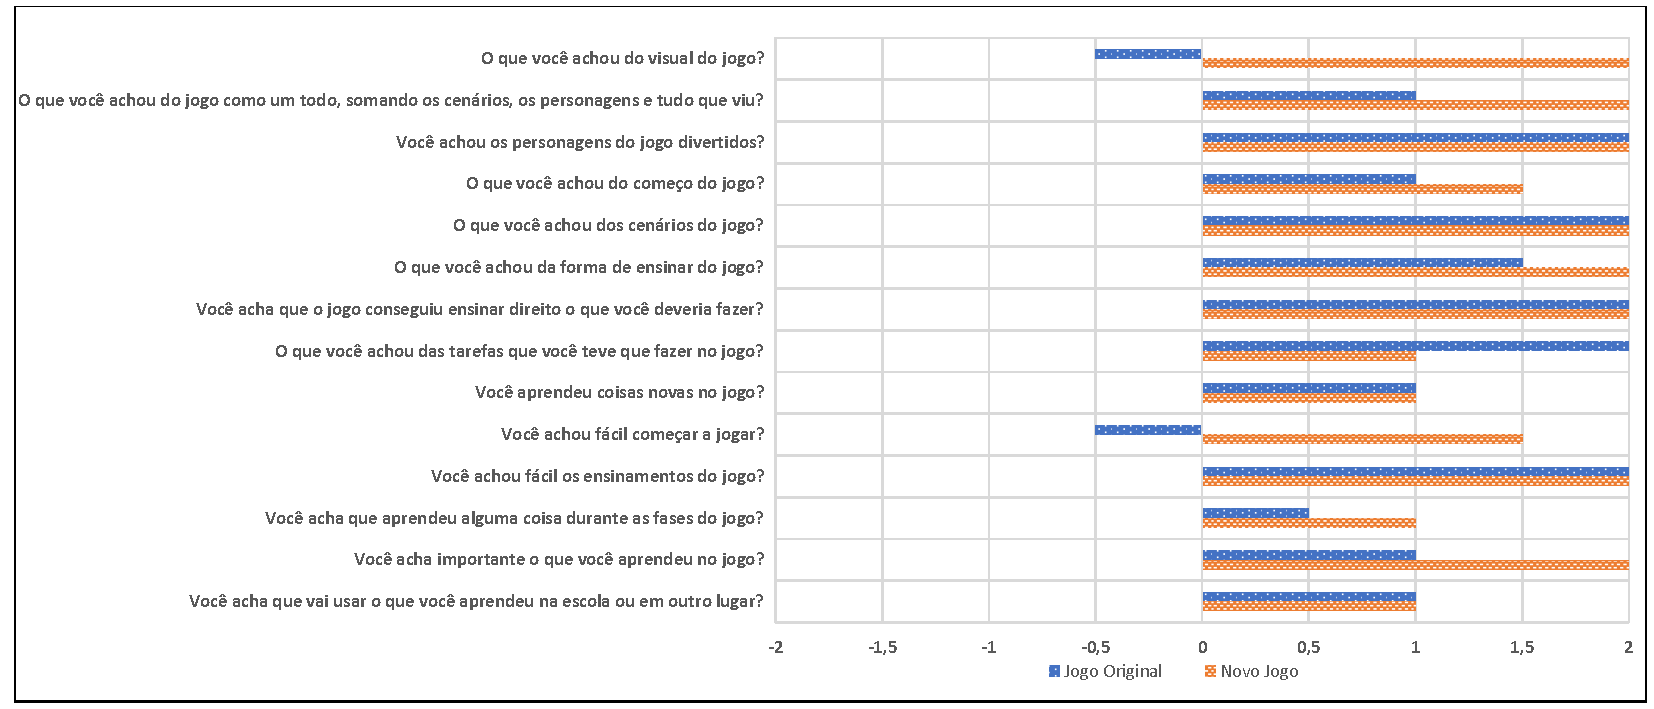
\includegraphics[width=\linewidth]{Resultados/Motivacao.pdf}
  \caption{Gráfico de medição da motivação do usuário}
  \label{fig:Motivacao}
\end{figure*} 


O gráfico da \cref{fig:Motivacao} traz a medição da \textbf{motivação} da primeira versão do jogo (\textbf{Infância Segura 1.0}) e a medição da \textbf{motivação} da nova versão desenvolvida pela presente pesquisa (\textbf{Infância Segura 2.0}). À esquerda da \cref{fig:Motivacao} encontram-se as respectivas perguntas do questionário. Quanto maior o valor (mais próximo de +2) melhor. Deste modo, o gráfico de \textbf{motivação}, mostra que a nova versão do jogo, supera a versão original em sete itens e se equipara em cinco.

O novo jogo proposto, demonstra perda de desempenho em relação a versão original na oitava questão do questionário. A oitava questão indaga os participantes sobre suas motivações no cumprimento das tarefas do jogo. Nesse sentido, o jogo original (\cref{subsecao:Jogar}) requer apenas uma tarefa ao jogador, para que ele comece a jogar, sendo tal tarefa a inserção do seu nome. Em contrapartida a nova versão do jogo (\cref{subsecao:JogoEducacional}), requer uma gama de outras tarefas além da inserção do nome pelo jogador, para que o mesmo possa finalmente adentrar no jogo. %Desta forma, já era previsível que o novo jogo poderia ter um desempenho inferior na oitava questão do questionário. 
Todavia, tais tarefas se fazem necessárias para a distinção de homônimos e para uma maior facilidade na gestão dos alunos pelo professor.

O jogo original teve desempenhos negativos no que diz respeito ao visual do jogo (primeira pergunta do questionário) e a facilidade em jogar o jogo (décima pergunta do questionário). Em termos estéticos, o jogo em questão apresenta o mesmo cenário de \textit{background} estático e não interativo. 

\newpage

Durante o questionário, os participantes foram indagados sobre a importância dos conteúdos aprendidos (décima terceira pergunta do questionário). Os resultados revelaram discrepâncias entre os jogos neste quesito, com o novo jogo apresentando um pontuação ligeiramente superior ao jogo original, salientando que as fases jogadas pelos participantes durante o experimento tinham como lição os mesmos ensinamentos em cada jogo, porém cada qual, da sua maneira. Aponta-se como um dos indícios para este resultado, que a forma pedagógica do novo jogo busca trazer mais seriedade e importância para os conteúdos ministrados em relação ao jogo original, vide por exemplo, a utilização do personagem de um Médico, trazendo assim mais autoridade e confiança aos jogadores sobre os assuntos abordados. 


 \begin{figure*}[ht]
  \centering
  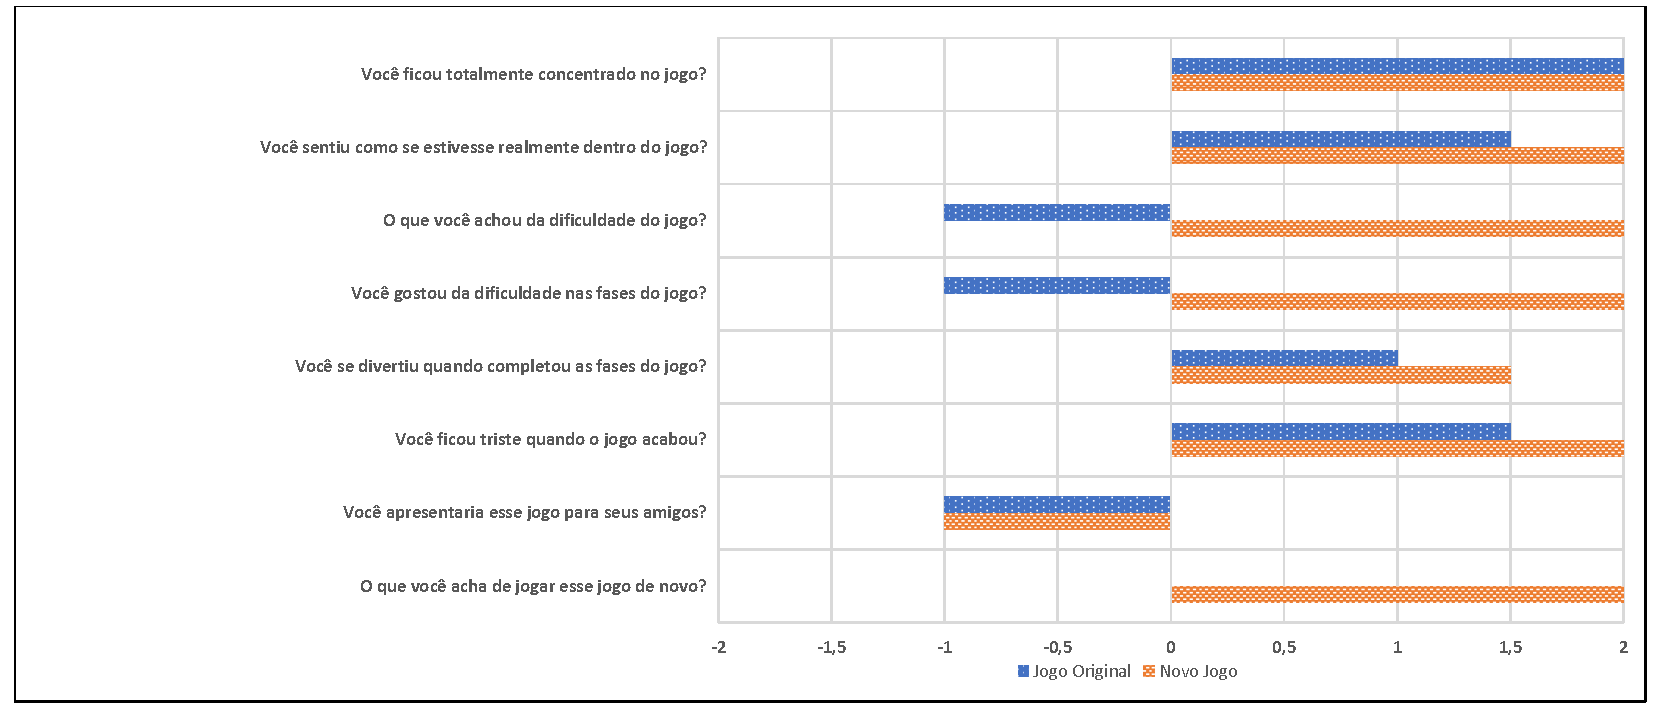
\includegraphics[width=1.05\linewidth]{Resultados/ExperienciaUsuario.pdf}
  %\vspace{-0.4 cm}
  \caption{Gráfico de medição da Experiência do Usuário}
  \label{fig:ExperienciaUsuario}
\end{figure*} 


O gráfico da \cref{fig:ExperienciaUsuario} apresenta as questões mensuradas sobre a \textbf{experiência dos usuários} em jogar o jogo. No gráfico, nota-se que o novo jogo (\textbf{Infânci Segura 2.0}) superou o jogo original (\textbf{Infânci Segura 1.0}) em seis questões e se equiparou em duas. %Dessas, salienta-se que ambos os jogos tiveram um baixo desempenho relacionado a divulgação dos mesmos.

Os resultados da \textbf{experiência dos usuários} revelam que os participantes acharam as fases jogadas no jogo original bastante difíceis. Na análise realizada, foi constatado que a exigência de um tempo de reação dos jogadores na \textbf{fase 1} e na \textbf{fase 2} foram fatores desmotivantes. O que acabou por configurar um desempenho negativo para a terceira e quarta questão do questionário sobre a \textbf{experiência dos usuários}.

\newpage

Em termos de \textit{level design} a \textbf{fase 1} do jogo original se apresenta como a fase mais difícil, pois nessa fase o jogador deve ser capaz de gerenciar três objetos simultaneamente (as duas caixas e as imagens), requisitando do jogador um grande esforço ao se iniciar o jogo. A \textbf{fase 2} se apresenta como a segunda fase mais fácil uma vez que a única preocupação do jogador é gerenciar as imagens que lhe são mostradas. A \textbf{fase 3} se apresenta como a segunda fase mais difícil, pois nela existe a preocupação de gerenciar dois objetos (tanto o avião, quanto as imagens que aparecem em tela). A \textbf{fase 4} é a última fase do jogo e se apresenta como a fase mais fácil, sendo que a única preocupação do jogador é responder as perguntas que lhe são feitas de forma a escolher apenas uma das duas opções apresentadas. Essa fase se demonstra mais fácil que a \textbf{fase 2}, uma vez que a \textbf{fase 2} requer um tempo de reação do usuário que na \textbf{fase 4} não é requerido.

A classificação de dificuldade das fases do jogo original foi feita com base na quantidade de elementos que são necessários serem gerenciados pelo jogador em cada fase. Desta forma, um desempenho inferior na décima questão do questionário já era esperado, vide o desapontamento infantil logo no início do jogo. 

Como resultado, o novo jogo  alcançou +25 pontos (94,64\%) na medição da \textbf{motivação}, contra +16 pontos (78,57\%) do jogo original, em uma escala de -28 pontos até +28 pontos. Já na escala de medição da \textbf{experiência dos usuários}, valorada de -16 pontos até +16 pontos, foram medidos 12,5 pontos (89,06\%) para nova versão, contra +3 pontos (59,37\%) para a versão original. %Ambos resultados promissores para um protótipo.

\newpage

\section{Considerações Finais}\label{secao:ConsideracoesFinais}

A violação sexual de crianças interfere diretamente no desenvolvimento da sexualidade saudável e nas dimensões psicossociais dos menores, causando danos muitas vezes irreversíveis. No Brasil, o número de vítimas violentadas alcançou sua maior alta histórica no ano de 2018. Em resposta a crescente quantidade de vítimas sexuais um jogo sério foi desenvolvido.

Em virtude da sensibilidade do tema tratado, o jogo foi analisado pela presente pesquisa para assegurar que os conteúdos ministrados estariam devidamente adequados para seu público alvo. Como resultado, o estudo da literatura revelou divergências entre o jogo educacional desenvolvido e recomendações para criação e modelagem de jogos, o que por sua vez culminou no desenvolvimento de um novo jogo.

Os jogos foram comparados, revelando a importância no cumprimento das bases da literatura, para o desenvolvimento de um jogo adequado ao público infantil. Os experimentos foram realizados com um número reduzido de participantes, o que prejudica a validação da pesquisa, porém garante uma supervisão particular para cada participante, assegurando assim seu bem estar. Como pesquisa futura, aponta-se a necessidade de testes com um maior número de participantes.

O novo jogo demonstrou maiores níveis de engajamento e aceitação em relação ao público avaliado. Nesse sentido, o presente trabalho relata e enfatiza a importância e os benefícios no cumprimentos das bases teóricas da literatura para a concepção e desenvolvimento de jogos.

\newpage

\section*{Agradecimentos}

O presente trabalho foi realizado com apoio da Coordenação de Aperfeiçoamento de Pessoal de Nível Superior - Brasil (CAPES) - Código de Financiamento 001.


\bibliography{RBCA_v2.0}                                %% Specify your .bib file name here, without the extension .bib
\end{document}

%The Revista Brasileira de Computação Aplicada (RBCA) is an \textbf{open-access journal} linked to the \href{http://ppgca.upf.br}{Graduate Program in Applied Computing (PPGCA)} of the \href{http://www.upf.br}{University of Passo Fundo}, Brazil. RBCA aims to provide to the scientific community article that presents an interdisciplinary perspective of the application of Computing in different areas of knowledge.

%This document is the \LaTeX{} template for RBCA journal manuscript submissions. \textcolor{red}{Submissions that do not use the format available in this template will be automatically rejected.} 

%\textbf{Articles submitted to RBCA should be between 8 and 15 pages and will be published electronically.} The languages accepted by RBCA are English (preferably) and Portuguese. We alert the authors that the preparation of the manuscript should be made carefully, both in its scientific content and in its grammatical correctness.

%There are essential commands in the preamble that you will need to modify for your manuscript. Define the paper language (``english'' or ``brazilian'') in \verb|\documentclass| command and specify your manuscript's category with the \verb|\papercat{...}| command. See the sample code in the preamble for a sample of how the title, author (names, orcid, affiliation, and e-mail) information can be specified. \textbf{If the paper is in Portuguese you need to inform the title in English using the} \verb|\titleother{...}| \textbf{command.} Information about this edition of RBCA and publication details of the paper will be filled out by the RBCA's editor.

%This template has been edited and validated in the \href{http://www.texstudio.org/}{TexStudio\copyright} program and the \href{https://www.overleaf.com/}{Overleaf\copyright} Collaborative Writing and Publishing System. Any questions or problems regarding this template report to the RBCA e-mail (\textcolor{blue}{rbca@upf.br}).

%The remainder of this current section will provide some sample \LaTeX{} code for various elements you may want to include in your manuscript.
